% Informe final · Ford Innovation Challenge III (AI Edition) · Data-Driven Powertrain Intelligence
% Compilar desde docs/informe/:   tectonic informe.tex
% Las figuras y las tablas generadas salen de:   python scripts/make_report_figures.py --config configs/report_figures.yaml
\documentclass[11pt,a4paper]{article}

\usepackage{fontspec}
\usepackage[spanish,es-noshorthands,es-tabla]{babel}
\setmainfont{texgyrepagella}[Extension=.otf,UprightFont=*-regular,BoldFont=*-bold,
  ItalicFont=*-italic,BoldItalicFont=*-bolditalic]
\setsansfont{texgyreheros}[Extension=.otf,UprightFont=*-regular,BoldFont=*-bold,
  ItalicFont=*-italic,BoldItalicFont=*-bolditalic]
\setmonofont{texgyrecursor}[Extension=.otf,UprightFont=*-regular,BoldFont=*-bold,Scale=0.95]

\usepackage[a4paper,top=2.2cm,bottom=2.2cm,left=2.3cm,right=2.3cm,headheight=14pt]{geometry}
\usepackage{microtype}
\usepackage{graphicx}
\usepackage{float}
\usepackage[section]{placeins}
\usepackage{booktabs,tabularx,longtable,multirow,array}
\usepackage{xcolor}
\usepackage{tikz}
\usetikzlibrary{arrows.meta,positioning,calc,fit,backgrounds,shapes.geometric}
\usepackage[most]{tcolorbox}
\usepackage{enumitem}
\usepackage{caption}
\usepackage{fancyhdr}
\usepackage{titlesec}
\usepackage[hidelinks]{hyperref}
\usepackage{bookmark}
\usepackage{listings}
\usepackage{multicol}
\lstset{basicstyle=\ttfamily\scriptsize,breaklines=true,breakatwhitespace=true,columns=fullflexible,
  keepspaces=true,frame=leftline,framerule=1.5pt,rulecolor=\color{fordblue!50},xleftmargin=8pt,
  commentstyle=\color{inksec},morecomment=[l]{\#},literate={á}{{\'a}}1 {é}{{\'e}}1 {í}{{\'i}}1
  {ó}{{\'o}}1 {ú}{{\'u}}1 {ñ}{{\~n}}1 {×}{{$\times$}}1 {'}{{'}}1,
  postbreak=\mbox{\textcolor{inksec}{$\hookrightarrow$}\space}}

% ---------------------------------------------------------------- colores (paleta de las figuras)
\definecolor{fordblue}{HTML}{2A78D6}
\definecolor{accent2}{HTML}{EB6834}
\definecolor{accent3}{HTML}{1BAF7A}
\definecolor{ink}{HTML}{0B0B0B}
\definecolor{inksec}{HTML}{52514E}
\definecolor{muted}{HTML}{A3A29D}
\definecolor{softbg}{HTML}{F4F7FC}
\definecolor{warnbg}{HTML}{FDF3EE}
\definecolor{rulec}{HTML}{D9D8D3}

% ---------------------------------------------------------------- estilo
\setlist{itemsep=2pt,topsep=4pt,parsep=0pt,leftmargin=1.4em}
\captionsetup{font=small,labelfont={bf,sf},format=hang,justification=raggedright,singlelinecheck=false}
\captionsetup[table]{position=top,skip=4pt}
\setlength{\parskip}{3pt}
\setlength{\parindent}{0pt}
\setlength{\emergencystretch}{2.5em}
\renewcommand{\arraystretch}{1.15}
\titlespacing*{\section}{0pt}{12pt}{6pt}
\titlespacing*{\subsection}{0pt}{9pt}{4pt}
\titlespacing*{\subsubsection}{0pt}{7pt}{3pt}
\setcounter{tocdepth}{2}
\renewcommand{\floatpagefraction}{0.8}
\renewcommand{\topfraction}{0.85}
\renewcommand{\textfraction}{0.1}
\titleformat{\section}{\sffamily\Large\bfseries\color{ink}}{\thesection}{0.8em}{}
\titleformat{\subsection}{\sffamily\large\bfseries\color{ink}}{\thesubsection}{0.7em}{}
\titleformat{\subsubsection}{\sffamily\normalsize\bfseries\color{ink}}{\thesubsubsection}{0.6em}{}
\pagestyle{fancy}
\fancyhf{}
\fancyhead[L]{\small\sffamily\color{inksec}Ford Innovation Challenge III · Data-Driven Powertrain Intelligence}
\fancyhead[R]{\small\sffamily\color{inksec}Equipo SOG}
\fancyfoot[C]{\small\sffamily\thepage}
\renewcommand{\headrulewidth}{0.4pt}

% marcas de dónde sale cada número
\newcommand{\tagtest}{\textsf{\footnotesize\textbf{\color{fordblue}[test]}}}
\newcommand{\tagdev}{\textsf{\footnotesize\textbf{\color{inksec}[dev]}}}
\newcommand{\fuente}[1]{\par\vspace{2pt}{\footnotesize\color{inksec}\textit{Fuente:} #1}}
\newcommand{\repo}[1]{{\footnotesize\ttfamily\begingroup\renewcommand{\_}{\textunderscore\allowbreak}#1\endgroup}}
\newcommand{\aprime}{(a$'$)}

\newtcolorbox{caja}[1][]{enhanced,breakable,colback=softbg,colframe=fordblue!60,boxrule=0.5pt,
  arc=2pt,left=8pt,right=8pt,top=6pt,bottom=6pt,fonttitle=\sffamily\bfseries,coltitle=ink,
  colbacktitle=softbg,attach title to upper={\par\smallskip},#1}
\newtcolorbox{limite}[1][]{enhanced,breakable,colback=warnbg,colframe=accent2!70,boxrule=0.5pt,
  arc=2pt,left=8pt,right=8pt,top=6pt,bottom=6pt,fonttitle=\sffamily\bfseries,coltitle=ink,
  attach title to upper={\par\smallskip},#1}

\hypersetup{pdftitle={Informe final · Ford FIC III · Equipo SOG},pdfauthor={Equipo SOG}}

\begin{document}

% ================================================================ portada + resumen ejecutivo
\begin{titlepage}
\thispagestyle{empty}
\vspace*{0.2cm}
{\sffamily\small\color{inksec} Ford Innovation Challenge III · AI Edition · Área: Data-Driven Powertrain Intelligence\par}
\vspace{0.7cm}
{\sffamily\fontsize{28}{34}\selectfont\bfseries\color{ink} Tu Ford te avisa antes\par}
\vspace{0.25cm}
{\sffamily\large\color{inksec} Predicción temprana de la degradación del filtro de partículas en los diésel conectados de
Ford\par}
\vspace{0.4cm}
{\normalsize Informe final del equipo SOG · Gonzalo · Santino · Octavio · 2 de octubre de 2026\par}
\vspace{0.7cm}
\phantomsection\addcontentsline{toc}{section}{Resumen ejecutivo}
\begin{caja}[title={Resumen ejecutivo}]
\small
\begin{itemize}
  \item \textbf{El problema.} El filtro de partículas (DPF) de los diésel se tapa según cómo se usa el auto, y hoy Ford se
    entera tarde: cuando se prende el testigo o el auto ya está en el taller. El desafío pide anticiparlo con la
    telemetría del auto conectado, con el mayor margen posible.
  \item \textbf{Lo que encontramos.} La telemetría deja huella: comparando contra sanos del mismo mercado, los autos que
    van a fallar pasan cada vez más tiempo en ralentí y con el motor frío. Pero los datos traían trampas que hacían que
    cualquier modelo pareciera mejor de lo que es (cohortes muestreadas en períodos distintos, una fecha del evento
    posterior al taller, un contador que se apaga). Las corregimos en un pipeline declarativo y trazable.
  \item \textbf{Lo que hicimos.} Cada 500 km, un modelo lee los últimos 1.000 km del auto y estima si falla en los
    próximos 3.000, sin ver nunca los 500 km previos a la falla. El finalista es una red recurrente (GRU) que lee la
    secuencia de viajes y de señales del filtro, más país, motor y modelo, en un ensamble de tres semillas. Un circuito
    convierte cada alerta en un consejo al conductor o en un llamado del concesionario, redactado por agentes de IA y
    controlado por un verificador en código.
  \item \textbf{Cuánto detecta} \tagtest{}. En 111 autos que nunca vio (103 con datos, 32 fallados), avisa a
    \textbf{\textasciitilde30\,\%} de las fallas con 5\,\% de autos sanos con falsa alarma (10 de 32, donde el azar da
    7\,\%), a \textbf{\textasciitilde40–50\,\%} con 10\,\% y a \textbf{\textasciitilde50–60\,\%} con 20\,\%. Con el umbral
    fijado antes, en desarrollo, las falsas alarmas reales quedan en 5,8 · 8,9 · 18,2\,\%.
  \item \textbf{Con cuánto margen} \tagtest{}. La primera alerta llega con una mediana de \textbf{\textasciitilde4.600 km,
    unos 3 meses}, antes de la falla registrada.
  \item \textbf{Cuánto cuesta.} Sin sensores nuevos y en CPU: \textasciitilde USD 0,07–0,10 por auto y por año para un
    millón de autos (estimación propia, a validar con Ford).
\end{itemize}
\end{caja}
\vfill
{\footnotesize\color{inksec} Repositorio \repo{ford-fic}, rama \repo{docs/informe}. Cada número trae su fuente en
\repo{docs/memoria/}, en el pitch o en un \repo{experiments/*/report.json}.\par}
\end{titlepage}

\tableofcontents

% ============================================================================ 0 · Cómo leer + criterios
\section*{Cómo leer este informe}
\addcontentsline{toc}{section}{Cómo leer este informe}

El informe sigue las siete secciones del documento de Ford. En cada una contamos qué entendimos, qué
encontramos en los datos y qué hicimos.

\begin{itemize}
  \item \tagtest{}: medido sobre los 111 autos del holdout, sorteados antes de mirar ninguna feature contra la
    etiqueta (103 con datos: 32 fallados y 71 sanos). Cada modelo se entrenó con todo el conjunto de desarrollo.
    \tagdev{}: validación cruzada agrupada por vehículo sobre los 446 autos de desarrollo. La demo, la explicabilidad
    y las auditorías son de dev.
  \item \textbf{Detección al X\,\%}: de los autos que fallan, cuántos reciben una alerta antes de la falla con un umbral
    fijado para que solo el X\,\% de los sanos tenga una falsa alarma. Una alerta son dos cortes seguidos sobre el umbral.
  \item \textbf{Azar}: el mismo puntaje permutado entre filas, conservando el largo del historial de cada auto.
  \item \textbf{Nada de accuracy}: con \textasciitilde6\,\% de filas positivas, “nadie falla” da 94\,\%. El PR-AUC por fila
    va al Anexo~\ref{anx:auditorias}, al lado del techo de cohorte.
\end{itemize}

\begin{table}[!htbp]
\centering
\caption{Los criterios de Ford (§5.1 y §5.2 del desafío) y dónde se responden.}
\label{tab:criterios}
\small
\begin{tabularx}{\textwidth}{@{}>{\raggedright\arraybackslash}p{3.4cm}>{\raggedright\arraybackslash}X>{\raggedright\arraybackslash}p{1.9cm}@{}}
\toprule
Criterio & Qué mostramos & Dónde \\
\midrule
Objetivo 5.1: anticipar con el mayor margen & \textasciitilde4.600 km (\textasciitilde100 días) de mediana en test, con
  500 km ciegos antes del evento; el puntaje sube hacia el evento & §\ref{sec:panel}, §\ref{sec:anticipacion} \\
Viabilidad técnica & Medido en un holdout congelado; GRU de \textasciitilde3.900 parámetros en CPU; demo funcionando;
  plan por etapas con piloto en sombra & §\ref{sec:viabilidad} \\
Costo & \textasciitilde USD 0,07–0,10 por auto y por año, sin sensores nuevos & §\ref{sec:costo} \\
Carácter innovador & Una métrica que separa \emph{qué auto} de \emph{cuándo}; red recurrente sobre la ventana; IA
  generativa con verificador en código; la perilla de falsas alarmas & §\ref{sec:innovacion} \\
Calidad del tratamiento de datos & Trampas de formato y de muestreo corregidas; atípicos con topes físicos; faltantes
  estructurales tratados como información; correcciones declaradas, holdout congelado y auditorías de leakage &
  §\ref{sec:datos}, Anexo~\ref{anx:auditorias} \\
Claridad para mostrar los datos & Curva de detección contra falsas alarmas con el azar dibujado; figuras con fuente;
  demo con tres pantallas y perilla & §\ref{sec:claridad} \\
Explicabilidad & En qué se apoya la GRU (permutación) y qué se le dice al conductor (comparación con la flota sana,
  filtrada por la física del DPF) & §\ref{sec:explicabilidad} \\
Pitch & La misma historia y los mismos números, en siete bloques y 29 minutos (\repo{docs/\allowbreak{}pitch/\allowbreak{}}) &
  §\ref{sec:claridad} \\
\bottomrule
\end{tabularx}
\end{table}

% ============================================================================ 1 · Descripción general
\section{Descripción general del desafío}
\label{sec:desafio}

\textbf{Título.} Ford pide una metodología de IA para predecir eventos de degradación de la eficiencia de combustión e
ingreso de oxígeno al motor, a partir de datos de vehículos conectados.

\textbf{Qué entendimos.} En un diésel, el componente que se degrada por el uso y afecta a la vez la combustión y el flujo
de gases es el filtro de partículas (DPF). El filtro atrapa el hollín y lo quema para limpiarse (regenera), pero para eso
necesita temperatura: un tramo de ruta con el motor caliente. Con viajes cortos, la regeneración empieza y no termina, el
hollín se acumula y, si sigue así, el auto entra en modo de protección y termina en el taller. Para el cliente, eso es un
testigo que nadie le explicó y la sensación de que nadie le avisó.

\textbf{Qué encontramos en los datos.}
\begin{itemize}
  \item \textbf{El evento es del filtro, con otro nombre.} \emph{TripSummary} no trae las columnas del DPF del anexo, pero sí
    \texttt{AirRegenerationStart/\allowbreak{}End} y \texttt{AirFilterStart/\allowbreak{}End}, que el anexo no menciona. Son la foto, al inicio y al
    final de cada viaje, de la acumulación (0–100) y de los nueve niveles de mensaje del filtro que trae
    \emph{DynamicInformation} (coinciden en el 99,8 y el 99,97\,\% de los pares). Ford no lo confirmó, así que hablamos de
    “nivel de acumulación del filtro”.
  \item \textbf{Es saturación por uso, no desgaste.} El evento cae a una mediana de \textasciitilde12.800 km, y la ceniza
    es un fenómeno de más de 100.000 km. Buscamos una carga irreversible medible (la premisa de un proceso de degradación
    tipo gamma) y no la hay. Eso orientó todo hacia los hábitos de manejo y el estado reciente del filtro.
  \item \textbf{No todo “uso indebido” se sostiene.} Comparando contra sanos \emph{del mismo mercado}, lo que crece hacia el
    evento es estar detenido con el motor en marcha y no llegar a temperatura. La velocidad y la fracción de viajes
    cortos no distinguen dentro del mercado: con la primera entrega, la velocidad parecía la mejor señal y era Colombia
    contra Chile.
\end{itemize}

\textbf{Qué hicimos.} Un modelo de deep learning que lee la secuencia de los últimos 1.000 km del auto y un producto que
convierte cada alerta en una acción. Al conductor no le hablamos de “uso indebido” ni de fallas: le hablamos de hábitos
que puede cambiar, comparados con autos sanos de su zona.

% ============================================================================ 2 · Contexto del proceso
\section{Contexto del proceso}
\label{sec:proceso}

\textbf{Qué entendimos.} La telemetría llega a la nube de forma continua, pero la degradación se identifica una vez
manifestada, en un service o cuando el cliente la reporta. El desafío se ubica en la posventa.

\textbf{Qué encontramos en los datos: el proceso reactivo está escrito en la telemetría.} La fecha registrada del evento
llega después del taller. En la primera entrega coincidía con la intervención (el cambio de aceite se concentraba en
±3 días). En la entrega v2, la fecha de los mismos autos cae una mediana de 14 días después, y en las dos semanas previas
ya aparecen el cambio de aceite y el ralentí largo de la regeneración forzada (1,5–1,8 veces la base). Después del evento,
además, el uso cambia: la fracción de viajes bajo régimen térmico baja en el 72\,\% de los autos.

\textbf{Qué hicimos.} Si el modelo viera el taller, haría la detección reactiva que Ford ya tiene. Por eso la referencia
del evento es la \textbf{fecha registrada menos 21 días}, el modelo nunca ve los \textbf{500 km previos} a esa referencia
(§\ref{sec:panel}) y nada posterior al evento entra a ninguna ventana. En la posventa, la alerta entra a un circuito que
termina en una acción (figura~\ref{fig:circuito}): con un hábito para nombrar, un consejo al conductor en la app; sin
hábito, un llamado del concesionario; si el riesgo sigue alto dos revisiones después, un escalamiento. El gerente de
posventa recibe cada lunes una bandeja priorizada y redactada, lista para aprobar.

\begin{figure}[!htbp]
\centering
\begin{tikzpicture}[
  node distance=4mm and 3.5mm,
  box/.style={draw=fordblue!70,fill=softbg,rounded corners=2pt,align=center,font=\sffamily\scriptsize,
    minimum height=10mm,text width=21mm,inner sep=2pt},
  pol/.style={box,draw=accent2!80,fill=warnbg},
  arr/.style={-{Stealth[length=2mm]},draw=inksec,thick}]
\node[box] (t) {\textbf{1 · Telemetría}\\viajes y señales del filtro};
\node[box,right=of t] (s) {\textbf{2 · Puntaje GRU}\\cada 500 km};
\node[box,right=of s] (a) {\textbf{3 · Alerta}\\2 cortes sobre el umbral de Ford};
\node[box,right=of a] (w) {\textbf{4 · Por qué}\\hábitos contra los sanos del mercado};
\node[pol,right=of w] (p) {\textbf{5 · Política}\\determinista, la define Ford};
\node[box,below=5mm of p] (g) {\textbf{6 · Agentes}\\redactan; un verificador controla};
\node[box,left=of g,text width=30mm] (u) {\textbf{Destinatarios}\\conductor · concesionario · posventa};
\node[box,left=of u,text width=30mm] (r) {\textbf{7 · Retorno del taller}\\monitoreo y reentrenamiento};
\draw[arr] (t) -- (s); \draw[arr] (s) -- (a); \draw[arr] (a) -- (w); \draw[arr] (w) -- (p);
\draw[arr] (p) -- (g); \draw[arr] (g) -- (u); \draw[arr] (u) -- (r); \draw[arr] (r) -| (t);
\end{tikzpicture}
\caption{El circuito de posventa: el modelo decide, el agente comunica y el código cuida lo que se dice.}
\label{fig:circuito}
\fuente{\repo{docs/\allowbreak{}pitch/\allowbreak{}presentacion-contenido.md} bloque 4; \repo{feat/\allowbreak{}demo-gru:PRODUCT.md}.}
\end{figure}

% ============================================================================ 3 · Definición del desafío
\section{Definición del desafío}
\label{sec:definicion}

\subsection{Desafío específico: anticipar el momento, sin hacer trampa}

\textbf{Qué entendimos.} Ford pide un modelo que anticipe, a partir de patrones históricos de uso y
variables de motor, \emph{el momento en que un vehículo se aproxima a un evento de degradación}, a tiempo
para una acción preventiva antes de que el cliente perciba el problema.

Esa frase tiene dos exigencias que tiran para lados distintos. \emph{Anticipar} pide no mirar los últimos
kilómetros antes de la falla, que es donde está la señal más fuerte. \emph{El momento} pide saber
\emph{cuándo}, y no solo \emph{qué auto}. La mayor parte del trabajo metodológico fue convertir esas dos
exigencias en una pregunta medible que no se pudiera ganar con atajos.

\subsubsection{La pregunta: un panel de cortes con gap de blanking}
\label{sec:panel}

Armamos un panel con una fila por par (vehículo, punto de corte). Los cortes caen cada
\textbf{Δ = 500 km} de odómetro. En cada corte, el modelo ve solo los últimos \textbf{W = 1.000 km} y
responde: ¿el evento cae entre \textbf{G = 500} y \textbf{G + H = 3.500 km} después del corte?
(figura~\ref{fig:panel}).

\begin{figure}[H]
\centering
\begin{tikzpicture}[x=1.55cm,y=1cm,font=\sffamily\scriptsize]
\fill[fordblue!18] (0,0) rectangle (1,0.7);
\fill[muted!35] (1,0) rectangle (1.5,0.7);
\fill[accent2!22] (1.5,0) rectangle (4.5,0.7);
\draw[inksec] (-0.6,0) -- (5.1,0);
\foreach \x/\l in {0/{−1.000},1/{corte},1.5/{+500},4.5/{+3.500}} {\draw[inksec] (\x,0) -- (\x,-0.1) node[below] {\l};}
\node at (0.5,0.35) {\textbf{W} · lo que mira};
\node at (1.25,0.35) {\textbf{G}};
\node at (3,0.35) {\textbf{H} · ¿falla acá?};
\draw[very thick,ink] (1,-0.15) -- (1,0.95);
\node[above] at (1,0.95) {punto de corte};
\node[below,text width=3.2cm,align=center] at (1.25,-0.45) {500 km ciegos: el modelo nunca los ve};
\node[right] at (5.1,0) {km};
\end{tikzpicture}
\caption{El planteo: ventana W hacia atrás, gap G y horizonte H hacia adelante. La etiqueta vale 1 si el
evento cae en el horizonte.}
\label{fig:panel}
\fuente{\repo{configs/\allowbreak{}data/\allowbreak{}panel\_v2.yaml}; \repo{docs/\allowbreak{}memoria/\allowbreak{}decisiones.md} (18-09).}
\end{figure}

\begin{itemize}
  \item \textbf{G = 500 km} es la regla antirreactiva. Sin ese gap, un modelo que mire los últimos kilómetros
    antes del evento memoriza los mensajes de “filtro sobrecargado” y reporta un número alto haciendo
    detección reactiva.
  \item \textbf{W = 1.000 km.} Con la primera entrega, cada 500 km más de ventana costaba unos tres eventos
    con positivo, y ventanas de 1.000, 2.000 y 3.000 km daban la misma métrica dentro del ruido.
  \item \textbf{H = 3.000 km} pone los positivos entre 500 y 3.500 km antes del evento, donde el perfil
    alineado muestra que la señal existe (§\ref{sec:eda}).
  \item \textbf{El eje es el odómetro} para cortar las ventanas, pero el evento se ordena por tiempo y no por
    km: la dispersión del logaritmo es 0,38 en edad contra 0,91 en odómetro. Quien maneja más llega al
    evento con más km, no antes. Por eso la anticipación se reporta en km y también en días aproximados.
  \item \textbf{Sanos emparejados por odómetro y por mes.} Los eventos se concentran en ciertos meses. Sin
    emparejar por mes, sumar tres columnas de calendario subía el ROC de 0,67 a 0,76; emparejando, de 0,57
    a 0,60 (primera entrega). El calendario no es el auto.
\end{itemize}

Con la entrega v2, el panel de desarrollo tiene 11.703 filas de 426 autos con cortes (135 fallados, 291
sanos) y 682 filas positivas: una tasa base de 0,058 por fila. Los autos sanos aportan en promedio 26,9
cortes y los fallados 28,8: las bolsas quedaron casi simétricas, algo que con la primera entrega no pasaba
(9,0 contra 18,3) y que obligó a corregir las métricas (abajo).

\subsubsection{Las reglas que no se negocian}

\begin{enumerate}
  \item \textbf{Gap de blanking}: el modelo nunca ve los 500 km previos al evento.
  \item \textbf{Split agrupado por vehículo}: un auto nunca está a la vez en entrenamiento y en validación.
    La lógica vive en un solo módulo (\repo{src/\allowbreak{}eval/\allowbreak{}splits.py}). Los folds se estratifican por la etiqueta a
    nivel vehículo, cruzada con mercado y motor, y la CV se repite tres veces.
  \item \textbf{Holdout congelado}: 111 autos sorteados una vez, antes de mirar ninguna feature contra la
    etiqueta. Todo lo que se mira es desarrollo; las filas de test no se tocan hasta tener el modelo elegido.
  \item \textbf{Features solo hacia atrás}: nada posterior al corte. Escalado e imputación se ajustan con el
    train de cada fold, dentro del pipeline.
  \item \textbf{Auditorías obligatorias} antes de aceptar un número (§\ref{sec:metricas}, Anexo~\ref{anx:auditorias}).
  \item \textbf{Nada se hardcodea}: paths, semillas e hiperparámetros salen de un YAML versionado.
\end{enumerate}

\subsubsection{Cómo medimos, y por qué cambiamos de métrica}
\label{sec:metricas}

Empezamos midiendo como manda el libro: PR-AUC por fila. Los primeros modelos daban números que parecían
buenos, hasta que nos preguntamos qué pasaría con un modelo que solo reconoce \emph{qué auto} falla, sin
saber nada del \emph{cuándo}.

\begin{caja}[title={El techo de cohorte}]
\small
Todas las filas positivas del panel están dentro de los cortes de autos que fallan. Un modelo que
puntúa cada fila con “¿este auto es de los que fallan?”, sin ninguna información del \emph{cuándo}, saca
\textbf{PR-AUC 0,177 y lift 3,03×} en el dev v2 (0,263 y 2,10× con la primera entrega). La meta inicial del
plan (lift de 1,6–2×) se alcanzaba sin anticipar nada. Ningún modelo superó ese techo: \textbf{un PR-AUC por
fila de este panel mide sobre todo \emph{qué auto} y muy poco \emph{cuándo}.}
\fuente{\repo{docs/\allowbreak{}memoria/\allowbreak{}decisiones.md}, cierre de F3 (20-09); \repo{src/\allowbreak{}eval/\allowbreak{}metrics.py::cohort\_ceiling}.}
\end{caja}

Tres mediciones independientes llegaron al mismo lugar con la primera entrega: colapsar el puntaje de cada
auto a su promedio \emph{mejoraba} la decisión por vehículo; la auditoría \aprime{} del modelo de control
daba negativa en las tres repeticiones; y un nulo que permuta la etiqueta dentro de cada auto quedaba por
encima del modelo. Desde entonces la pregunta que decide es una sola:

\begin{quote}
\emph{De los autos que van a fallar, ¿a cuántos les avisamos a tiempo si solo permitimos una cantidad fija
de falsas alarmas entre los autos sanos?}
\end{quote}

\begin{itemize}
  \item \textbf{Detección por auto} con umbral exacto: para cada presupuesto b (2 a 30\,\% de los sanos con
    alguna falsa alarma), el umbral es el menor que deja a lo sumo b de los sanos alertados. Una alerta son
    \textbf{dos cortes seguidos} sobre el umbral. El criterio primario es la detección media al 5, 10, 15
    y 20\,\%.
  \item \textbf{Contra el azar, con el mismo historial}: el puntaje permutado entre filas, 200 veces. Con la
    primera entrega, las bolsas asimétricas “detectaban” 10\,\% al 5\,\% sin ninguna señal; toda métrica que
    dependa del largo del historial se compara contra un nulo que lo conserve.
  \item \textbf{Contra la celda mercado × motor}: la tasa de fallas de la celda del auto, calculada sin él.
    Tres celdas (Chile × ENG\_2, Colombia × ENG\_2 y Brasil × ENG\_3) concentran 117 de los 135 fallados de
    dev. Esa regla, sin mirar un viaje, detecta 18 · 33 · 62\,\% al 5 · 10 · 20\,\% \tagdev{}.
  \item \textbf{Fuera de muestra}: el umbral se fija con los sanos de los otros folds y se mide la tasa de
    falsas alarmas que realmente produce.
  \item \textbf{Bootstrap pareado por vehículo} para comparar dos modelos, con 1.000 a 2.000 réplicas.
  \item \textbf{AUC dentro de mercado × motor}: solo compara pares de autos de la misma celda. La diferencia
    con el AUC agrupado es composición de la muestra.
\end{itemize}

Para elegir candidatos, además, cada comparación nueva gastaba un lugar de un \emph{presupuesto de
comparaciones}: con unos 12 eventos por fold, sumar candidatos sobre la marcha garantiza que “el mejor” sea
ruido. Las variantes importantes se preregistraron por escrito antes de medirlas (\repo{docs/\allowbreak{}memoria/\allowbreak{}*preregistro*}).

\subsection{Impacto operativo}

\textbf{Qué entendimos.} No anticipar estos eventos afecta la satisfacción del cliente, sube los costos de
garantía y reparación, reduce la vida útil percibida y desordena la planificación de mantenimiento de la red
de concesionarios.

\textbf{Qué hicimos con cada punto.}
\begin{itemize}
  \item \textbf{Satisfacción}: un aviso a tiempo, en lenguaje humano y con algo concreto para hacer. Si el
    auto no iba a fallar, el conductor igual recibió un consejo que le sirve.
  \item \textbf{Garantía y reparación}: la alerta llega con una mediana de unos tres meses de margen
    \tagtest{}, tiempo para cambiar un hábito o programar un turno en vez de una urgencia. Cuántas fallas se
    evitan no se puede medir con estos datos: es la métrica central del piloto (§\ref{sec:viabilidad}).
  \item \textbf{Planificación de concesionarios}: la bandeja semanal prioriza los casos, y la perilla deja que
    Ford elija cuántas alertas acepta según su capacidad y el costo de cada una.
\end{itemize}

% ============================================================================ 4 · Datos técnicos relevantes
\section{Datos técnicos relevantes}
\label{sec:datos}

Esta sección es la respuesta al criterio de \emph{calidad del tratamiento de datos}. Contamos qué llegó, qué
trampas tenía, qué descartamos y por qué, y cómo quedó trazado cada paso. Las dificultades son parte del
resultado: varias cosas que creíamos saber con la primera entrega dejaron de ser ciertas con la segunda.

\subsection{Las tres tablas: lo que prometía el anexo y lo que llegó}

Ford describe tres tablas (anexo 7 del desafío): \emph{Trip Summary} (estado del vehículo al inicio y al
final de cada viaje), \emph{DynamicInformation} (estados en cada envío de datos) y \emph{Vehicle General
Information} (datos estáticos). Llegaron como seis CSV, cada tabla partida en dos cohortes de muestreo:
vehículos con evento registrado (\emph{Failed}) y sin evento (\emph{NotFailed}).

\begin{table}[H]
\centering
\caption{Los archivos de las dos entregas. La telemetría de los sanos de la entrega v2 es byte a byte la de
la entrega 1: todo lo nuevo está en la estática y en los archivos de fallados.}
\label{tab:archivos}
\small
\begin{tabular}{@{}llrrl@{}}
\toprule
Tabla & Cohorte & Filas, entrega 1 (15-09) & Filas, entrega v2 (26-09) & ¿Igual? \\
\midrule
Estática & fallados & 378 & 298 & no \\
Estática & sanos & 742 & 768 & no \\
Viajes (\emph{TripSummary}) & fallados & 947.477 & 934.463 & no \\
Viajes (\emph{TripSummary}) & sanos & 1.583.958 & 1.583.958 & sí \\
Señales (\emph{DynamicInformation}) & fallados & 4.202.484 & 3.595.216 & no \\
Señales (\emph{DynamicInformation}) & sanos & 6.415.333 & 6.415.333 & sí \\
\bottomrule
\end{tabular}
\fuente{\repo{docs/\allowbreak{}memoria/\allowbreak{}f9-entrega-v2.md} §1 y \repo{f1-datos-reales.md}; reproduce
\repo{scripts/\allowbreak{}compare\_deliveries.py}.}
\end{table}

\textbf{Qué encontramos al contrastar contra el anexo} (detalle en el Anexo~\ref{anx:tablas}):
\begin{itemize}
  \item \textbf{\emph{TripSummary} trae 25 de las 40 columnas documentadas.} Faltan 19: GPS (4), elevación (2),
    presión de neumáticos (8), hollín de regeneración manual (2), autonomía (1) y el DPF por su nombre (2).
    Aparecen 4 que el anexo no menciona: \texttt{AirFilterStart/\allowbreak{}End} y \texttt{AirRegenerationStart/\allowbreak{}End}, que
    son el DPF con otro nombre (§\ref{sec:desafio}).
  \item \textbf{\emph{DynamicInformation} y la estática cierran} (7 y 7 columnas), con renombres cosméticos:
    \texttt{Vin} → \texttt{VehicleCode}, \texttt{SalesCountryCd} → \texttt{SalesCountry\_cd}. No hay VIN: el
    único identificador es \texttt{VehicleCode}, y el join entre las tres tablas cierra.
  \item \textbf{El evento no está marcado fila a fila}: sale del vehículo. \texttt{IdentificationDate} está en
    el 100\,\% de los fallados y es nula en el 100\,\% de los sanos. \textbf{La cohorte es la etiqueta}, y por
    eso nunca entra como variable.
  \item \textbf{\texttt{Regenerations} no es un booleano}: es el texto literal \texttt{“Regeneration”} que marca
    una fila. Declararla numérica la convertía en nula en silencio.
  \item Los seis archivos vienen con BOM: si no se leen como \texttt{utf-8-sig}, la primera
    columna sale con el BOM pegado al nombre y el join falla.
\end{itemize}

\subsection{Equipos o sistemas existentes: el histórico por vehículo}

\textbf{Qué entendimos.} El documento promete un histórico de recolección por vehículo, con autos con y sin
degradación, y deja la periodicidad y el volumen a confirmar.

\textbf{Qué encontramos.} Hay historial de sobra para ventanas de varios miles de km. Con la primera
entrega, la mediana por vehículo era de \textasciitilde2.000 viajes, \textasciitilde7.000–8.000 señales,
\textasciitilde17.000–21.000 km de odómetro final y 400–470 días de historia. \emph{TripSummary} tiene una
fila por viaje y \emph{DynamicInformation} una por mensaje de la ECU. Tres cosas del “sistema” importan más
que el volumen:
\begin{itemize}
  \item \textbf{Las dos cohortes se extrajeron en fechas distintas}: los viajes de fallados de la entrega v2
    llegan al 24-09-2026 y los de sanos terminan el 14-09-2026. Hay 16.911 viajes de fallados posteriores al
    último de un sano. Un modelo que los viera aprendería “si hay datos después del 14-09, es un fallado”.
  \item \textbf{Un contador se apagó}: el marcador \texttt{Regenerations} de \emph{DynamicInformation} deja de
    registrarse el 25-05-2026 para toda la flota (cero marcadores de junio en adelante contra unas 2.000
    caídas de nivel por mes en los viajes).
  \item \textbf{Las fechas mezclan dos formatos} en el mismo archivo (con y sin microsegundos). Sin declarar
    ISO 8601, pandas anula las del segundo formato en silencio: 4.464 inicios de viaje, 3.298 fines y 18.124
    timestamps de señales. El crudo tiene cero nulos.
\end{itemize}

\subsection{Restricciones técnicas: anonimización y renombres}
\label{sec:restricciones}

\textbf{Qué entendimos.} Las variables vienen renombradas y, cuando corresponde, anonimizadas, para preservar
la confidencialidad.

\textbf{Qué encontramos y qué hicimos.}
\begin{itemize}
  \item Los vehículos son \texttt{VEH\_xxxx}, los motores \texttt{ENG\_1..3} y las series \texttt{MODEL\_x}. Los
    países venían como \texttt{CNTRY\_1..5}; la entrega v2 trae el código ISO (ARG, BRA, CHL, COL, PER) y la
    ciudad de venta.
  \item El DPF llegó como “Air Filter” y “Acumulation”. Lo tratamos como \emph{nivel de acumulación del
    filtro, escala 0–100}, que siempre es correcto, sin afirmar una semántica que Ford no confirmó.
  \item Sin GPS ni elevación por viaje, las features de altura previstas murieron. Con la entrega v2 probamos
    la altura de la ciudad de venta (geocodificada desde una fuente pública): va en la dirección de la física,
    pero no se separa del cero (§\ref{sec:eda}). Sin presión de neumáticos tampoco hay features de esa familia.
\end{itemize}

\subsection{Lo que encontramos: las trampas de los datos}
\label{sec:trampas}

Cada una de estas trampas rompe algo en silencio: no hay error, solo un número mejor de lo que debería.

\begin{table}[H]
\centering
\caption{Las trampas que encontramos, cómo las vimos y qué hicimos.}
\label{tab:trampas}
\scriptsize
\begin{tabularx}{\textwidth}{@{}>{\raggedright\arraybackslash}p{2.9cm}>{\raggedright\arraybackslash}X>{\raggedright\arraybackslash}p{4.2cm}@{}}
\toprule
Trampa & Cómo la vimos & Qué hicimos \\
\midrule
Dos listas muestreadas en períodos de producción distintos &
  En la entrega v2, antes del 20-01-2025 solo hay fallados (93) y después de julio de 2025 solo hay sanos
  (341), contra unos 50 eventos esperados por su exposición. Sumando esos autos, la fecha de producción sola
  separa fallados de sanos dentro del mercado con AUC 0,87 &
  Universo = período común, 20-01 a 31-07-2025 (§\ref{sec:universo}) \\
La fecha registrada es posterior al taller &
  Cambio de aceite y ralentí largo (1,5–1,8× la base) en las dos semanas previas a la fecha v2; la fecha v1
  de los mismos autos cae una mediana de 14 días antes &
  Referencia del evento = fecha − 21 días \\
El contador de regeneraciones se apaga &
  Cero marcadores desde el 25-05-2026 en toda la flota. Su correlación con la etiqueta (0,317) era
  calendario: contadas desde las caídas del nivel, cae a 0,072 &
  Fuera del modelo (\texttt{aux\_}); regeneraciones = caídas de \texttt{AirRegeneration} de al menos 15 puntos \\
13 autos con dos códigos &
  Mismos viajes bajo dos identificadores consecutivos (Jaccard 1,0 sobre fecha y odómetro de cada viaje);
  en la entrega 1, además, cada código aparecía en las dos cohortes &
  Se colapsan a 13 vehículos antes de cualquier split, con la etiqueta a favor del fallado \\
Formato de la entrega v2 &
  Columna del evento renombrada solo en fallados; \texttt{ProductionDay} de fallados contado desde otro origen
  (+538 días exactos en los 15 códigos comunes); una fila por evento (19 autos con 2 eventos, uno con 4);
  26 filas repetidas en sanos; extracción de fallados diez días más larga &
  Corrección al leer, declarada en \repo{raw\_sources.yaml} (\texttt{rename}, \texttt{offsets},
  \texttt{truncate\_after}) y probada en \repo{check\_setup.py} \\
La tasa por país depende de cómo se armó la lista &
  Va de 0\,\% (PER) a 48\,\% (COL), en el orden inverso de cuántos fallados sin fecha sacó Ford de cada
  mercado &
  Toda comparación fallado/sano, dentro del mercado; todo AUC, también dentro de mercado × motor \\
\texttt{ENG\_3} nunca fallaba (entrega 1) &
  0 fallados entre 268 \texttt{ENG\_3}: muestreo, no física. En la v2 tiene 47 eventos, 46 en Brasil &
  Fuera del modelo con la entrega 1; vuelve con la v2, reportando siempre dentro de la celda \\
Después del evento el uso cambia &
  Bajo régimen baja en el 72\,\% de los autos y la velocidad sube en el 79\,\% &
  Nada posterior al evento entra a ninguna ventana \\
\bottomrule
\end{tabularx}
\fuente{\repo{f9-entrega-v2.md}, \repo{f9-universo-v2.md}, \repo{f9-eda-v2.md}, \repo{f1-clones-vehiculos.md},
\repo{f1-sesgo-eng3.md}, \repo{f2-eda-revision-y-features.md} §2.1.}
\end{table}

\textbf{Una pregunta que solo Ford puede contestar.} Entre la entrega 1 y la v2 desaparecieron 285 códigos
de fallados. 278 tenían la fecha por defecto (\texttt{IdentificationDate} igual a los días hasta la venta):
Ford no corrigió esas fechas, sacó a esos autos. No sabemos si eran fallas reales sin fecha o un error de la
consulta. Importa porque se concentran por mercado, y explican en parte por qué la tasa de fallas cambia
tanto de un país a otro.

\subsection{Limpieza, faltantes y atípicos}
\label{sec:limpieza}

\begin{table}[H]
\centering
\caption{Valores imposibles, faltantes y columnas con trampa, y cómo se trataron.}
\label{tab:limpieza}
\scriptsize
\begin{tabularx}{\textwidth}{@{}>{\raggedright\arraybackslash}p{3.2cm}>{\raggedright\arraybackslash}X>{\raggedright\arraybackslash}p{4.6cm}@{}}
\toprule
Problema & Magnitud & Tratamiento \\
\midrule
Velocidad imposible & hasta 135.600 km/h (0,03\,\% de los viajes sobre 200 km/h) &
  Velocidad recalculada como km/duración, con tope físico de 200 km/h \\
\texttt{KilometerPerHour} nulo & \textasciitilde33\,\% en v2, \emph{exactamente} en los viajes de 0 km (100\,\% de esas
  filas, 0,05\,\% del resto); donde existe, es km/duración con Pearson 0,99999 &
  No se imputa: esas filas son ralentí y se cuentan aparte \\
Viajes de 0 km (ralentí) & 33,4\,\% de las filas de \emph{TripSummary} (v2) &
  Toda fracción “de viaje” se calcula entre los que se mueven; el ralentí es una señal propia, la que más
  anticipa \\
Temperaturas y duraciones extremas & −73 °C de ambiente, viajes de 20 días, viajes de −230 km (< 0,05\,\% cada
  uno) & Topes físicos fijos, no cuantiles (los cuantiles dependerían del train de cada fold): motor y
  refrigerante [−40, 130] °C, ambiente [−40, 60] °C, duración [0, 1.440] min \\
Nivel de combustible & supera 100 en el 10,5\,\% de los viajes (hasta 103,5) & No se recorta a [0, 100]: se
  trata como índice relativo \\
Vida del aceite & igual al inicio y al final del viaje en el 100\,\% de los casos & La feature es la pendiente
  del nivel contra el odómetro en la ventana, no la suma de deltas \\
Odómetro de señales nulo & 11,15\,\% en la entrega 1, concentrado en 9 vehículos (mediana por vehículo
  0,00\,\%); 0,5\,\% en los fallados v2 & La ventana se ubica por el odómetro de los viajes, que está
  prácticamente completo (8 filas nulas) \\
Retrocesos del odómetro & 165 viajes con km negativos en 24 vehículos (entrega 1) & Esos viajes y los que no
  tienen odómetro se descartan: no tienen una posición confiable en el eje de km \\
Umbral de regeneración & con caídas de 5 puntos, el saldo de caídas no sigue la acumulación medida
  (correlación 0,005) & Se exige una caída de al menos 15 puntos (correlación mediana 0,45 dentro del auto) \\
Escala de acumulación & llega a 100 (0,58\,\% de los fines de viaje); 95 es un escalón con masa, no el tope &
  Saturado = nivel ≥ 95 \\
Bins sin viajes (secuencia) & tramos de 50 km sin registros & Un canal de cobertura (cantidad de viajes y de
  registros) más arrastre del último valor dentro de la misma ventana: un tramo vacío no es “cero ralentí” \\
\bottomrule
\end{tabularx}
\fuente{\repo{f2-calidad-columnas-dev.md}, \repo{f1-calidad-odometro.md}, \repo{f2-umbral-regeneraciones.md},
\repo{f2-eda-revision-y-features.md} §2, \repo{configs/\allowbreak{}data/\allowbreak{}features\_v1.yaml} (\texttt{clip}, \texttt{thresholds}),
\repo{configs/\allowbreak{}data/\allowbreak{}panel\_seq\_trips\_v2\_estaticas.yaml}.}
\end{table}

\textbf{Faltantes que no se imputan.} Dos faltantes son estructurales y los tratamos como información:
la velocidad nula en los viajes de 0 km (es ralentí, no un dato perdido) y la fecha del evento nula en los
sanos (es la etiqueta, no una covariable). El resto de la imputación (mediana) y el escalado se ajustan con
el train de cada fold, dentro del \texttt{Pipeline}, nunca sobre el panel entero.

\subsection{El universo del estudio y el holdout}
\label{sec:universo}

\begin{figure}[H]
\centering
\begin{tikzpicture}[font=\sffamily\scriptsize,
  b/.style={draw=fordblue!70,fill=softbg,rounded corners=2pt,align=center,minimum height=10mm,inner sep=3pt},
  xb/.style={draw=muted,fill=white,rounded corners=2pt,align=left,inner sep=3pt,text width=4.6cm},
  arr/.style={-{Stealth[length=2mm]},draw=inksec,thick}]
\node[b,text width=3.4cm] (all) {\textbf{991 vehículos} con etiqueta\\en la entrega v2};
\node[b,text width=3.4cm,below=7mm of all] (uni) {\textbf{557 vehículos} · 177 eventos\\producidos 20-01 a 31-07-2025\\ARG, BRA, CHL, COL, PER};
\node[b,text width=2.6cm,below left=8mm and -1.2cm of uni] (dev) {\textbf{446 desarrollo}\\141 eventos};
\node[b,text width=2.6cm,below right=8mm and -1.2cm of uni,draw=accent2!80,fill=warnbg] (test) {\textbf{111 test, bajo llave}\\36 eventos};
\node[xb,right=12mm of all] (out) {\textbf{434 fuera del universo}\\ 92 fallados producidos antes del 20-01-2025 (sin ningún sano de su época)\\ 341 sanos producidos después del 31-07-2025 (0 fallados contra \textasciitilde50 esperados)\\ 1 fallado de PRY (mercado sin sanos)};
\draw[arr] (all) -- (uni); \draw[arr] (uni) -- (dev); \draw[arr] (uni) -- (test);
\draw[arr,muted] (all) -- (out);
\end{tikzpicture}
\caption{Del dataset al universo y al holdout. El holdout se sorteó una vez (semilla 42), estratificado por
evento × mercado × motor, antes de mirar ninguna feature contra la etiqueta.}
\label{fig:embudo}
\fuente{\repo{docs/\allowbreak{}memoria/\allowbreak{}f9-universo-v2.md} §3–§4; \repo{configs/\allowbreak{}data/\allowbreak{}test\_split.yaml}; reproduce
\repo{scripts/\allowbreak{}make\_test\_split.py}.}
\end{figure}

\textbf{Por qué el período de producción.} Es la misma regla simétrica que usamos con la primera entrega,
aplicada en otro eje: se conserva el período donde las dos cohortes se muestrearon. Un sano producido en
octubre de 2025 no es un negativo verificable si en esa época no se registró ninguna falla. El equipo propuso
sacar el recorte para no tirar 433 autos, y lo probamos de punta a punta (990 vehículos): con los autos de
afuera, la fecha de producción sola separaba fallados de sanos con AUC 0,87 dentro del mercado, y los
modelos ordenaban \emph{peor} a los autos comparables (survival stacking, de 0,571 a 0,471 dentro de mercado
× motor). Volvimos a la ventana. Cortar por km no evita el problema, porque lo sesgado es quién entra en la
muestra, no el eje.

\textbf{Lo que costó re-sortear.} Con la entrega v2 el holdout se volvió a sortear con la misma semilla: el
universo, las etiquetas y los estratos cambiaron enteros. 36 de los 111 autos del test nuevo estaban en el
desarrollo de la entrega 1 (13 con evento) y se habían mirado durante el análisis. Por eso el test se
reporta también sin ellos (§\ref{sec:test}).

\begin{table}[H]
\centering
\caption{Qué cambió al rehacer todo con la entrega v2. Lo que no se sostuvo, se dice.}
\label{tab:v1v2}
\scriptsize
\begin{tabularx}{\textwidth}{@{}>{\raggedright\arraybackslash}X>{\raggedright\arraybackslash}X@{}}
\toprule
Con la entrega 1 (364 autos, 2 mercados, 80 eventos) & Con la entrega v2 (557 autos, 5 mercados, 177 eventos) \\
\midrule
La velocidad baja antes de la falla: la señal más fuerte & Desaparece dentro del mercado: era Colombia (lenta,
falla) contra Chile \\
No hay trayectoria: el exceso de ralentí no crece hacia el evento & Sí crece: 0,60 → 0,64 → 0,76 \\
El registro de eventos tiene una ventana de calendario (sep-2025 a mar-2026) & No hay ventana: era de la
extracción vieja (el mes calendario no agrega nada, p = 0,16) \\
El riesgo crece con la edad sin parar & Sube hasta \textasciitilde4 meses desde la venta (0,34 → 2,11 → 3,37
eventos por 100 autos-mes) y después queda en \textasciitilde3–4 \\
\texttt{ENG\_3} nunca falla y queda afuera & \texttt{ENG\_3} falla (46 de sus 47 eventos en Brasil) y entra \\
La fecha del evento es la intervención & La fecha cae \textasciitilde2 semanas después: se corre 21 días \\
Rasgo temprano post-venta, AUC \textasciitilde0,62–0,68 & Se sostiene con 3× los eventos y en 5 mercados
(\textasciitilde0,60–0,64) \\
Finalista: survival stacking con la ventana del registro (K2), \textasciitilde15–17\,\% al 5\,\% & K2 pierde su
corrección (la ventana) y no aprueba \aprime{}; los secuenciales pasan adelante \\
\bottomrule
\end{tabularx}
\fuente{\repo{f9-eda-v2.md} §1; \repo{decisiones.md} (26-09); \repo{f9-remedicion-v2.md}.}
\end{table}

\subsection{Las features: qué entró, qué no y por qué}
\label{sec:features}

El modelo recibe la ventana de 1.000 km de dos formas, según la familia de modelo (diccionario completo en
el Anexo~\ref{anx:features}):

\begin{itemize}
  \item \textbf{53 features agregadas} (modelos tabulares y de supervivencia), en cuatro familias:
    \textbf{A · térmica y trayectos cortos} (17: ralentí, viajes bajo régimen, temperaturas, arranques en frío,
    viajes encadenados, distancia y duración), \textbf{B · regeneración} (15: regeneraciones por 1.000 km
    contadas desde las caídas del nivel, distancia entre regeneraciones, nivel residual, saturación, avisos del
    filtro al fin del viaje), \textbf{C · uso} (6: velocidad recalculada, fracción urbana, viajes y km por día,
    reposo entre viajes) y \textbf{D · severidad} (13: tasas de mensajes del filtro por 1.000 km, vida del
    aceite y su pendiente, consumo), más 2 controles de cobertura de la ventana.
  \item \textbf{La secuencia} (modelos recurrentes): la ventana en 20 tramos de 50 km × 15 canales. 9 canales
    salen de las señales (registros, cobertura, acumulación media y máxima, cuánto sube, caídas por
    regeneración, y tres fracciones de avisos) y 6 de los viajes (cantidad, ralentí, bajo régimen entre los
    que se mueven, velocidad, km y duración por viaje). Más país, motor y serie como estáticas.
\end{itemize}

\begin{table}[H]
\centering
\caption{Qué datos entraron al modelo y cuáles quedaron solo para auditar.}
\label{tab:entro}
\scriptsize
\begin{tabularx}{\textwidth}{@{}>{\raggedright\arraybackslash}p{4.4cm}>{\raggedright\arraybackslash}p{2.6cm}>{\raggedright\arraybackslash}X@{}}
\toprule
Dato & Decisión & Por qué \\
\midrule
Viajes: ralentí, temperaturas, duración, nivel del filtro, regeneraciones reconstruidas & entra & Es el uso y el
  estado del filtro, siempre hacia atrás del corte \\
Mensajes del filtro & entra como tasas por 1.000 km & Severidad. Sin el gap serían casi la definición del
  evento: por eso el gap existe \\
Mercado, motor y serie & entran (v2) & Aportan la tasa de su celda y no orden entre autos: todo modelo que los
  usa se reporta también dentro de mercado × motor \\
Fecha de producción, de venta, días hasta la venta & solo auditoría (\texttt{aux\_}) & Miden la cohorte de
  muestreo, no el auto \\
Temperatura ambiente & solo auditoría & Deriva con el mes y con el lugar: los fallados viven en lugares más
  fríos que los sanos de su mercado \\
Marcador \texttt{Regenerations} y \texttt{DistanceBetweenRegenerations} & solo auditoría & Se cortan el
  25-05-2026: miden el calendario \\
Interrupciones de regeneración & no se construye & 1 mensaje de cada 100.000 \\
Altura de la ciudad de venta & no entra & En la dirección de la física (RR 1,30 por cada 1.000 m, IC95
  [0,93; 1,81]) pero no significativa, y la ciudad de venta no es la de uso \\
Los 433 autos fuera del período común & fuera de toda comparación fallado/sano & Con ellos la fecha de
  producción domina (AUC 0,87) \\
\bottomrule
\end{tabularx}
\fuente{\repo{decisiones.md} (18-09 y 26-09); \repo{f9-eda-v2.md} §I; \repo{configs/\allowbreak{}data/\allowbreak{}features\_v1.yaml}.}
\end{table}

\subsection{Qué dicen los datos: el análisis exploratorio}
\label{sec:eda}

Todo lo de esta sección es de desarrollo \tagdev{} y compara fallados contra sanos \emph{del mismo mercado}.
En la entrega v2 una comparación agrupada mezcla mercado con señal: con cinco mercados de tasas tan
distintas, la versión agrupada infla lo que en realidad es país (por ejemplo, la fracción de avisos de filtro
anormal pasa de 0,52 dentro del mercado a 0,58 agrupada).

\begin{figure}[H]
\centering
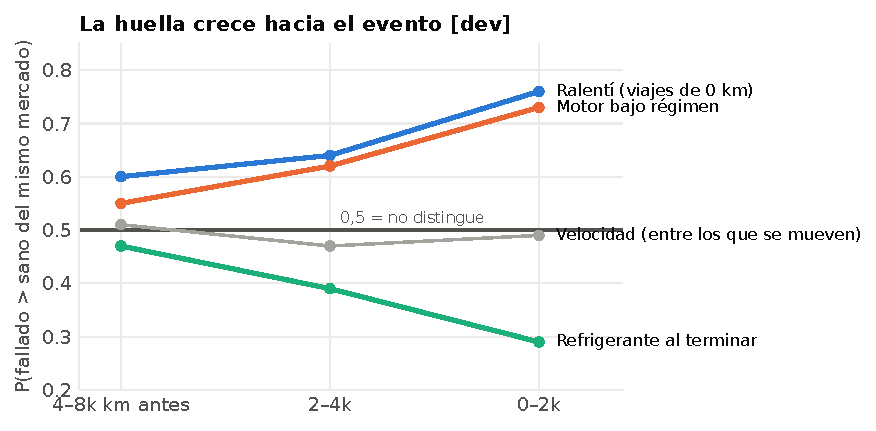
\includegraphics[width=0.9\textwidth]{figuras/perfil_evento.pdf}
\caption{Probabilidad de que un auto que va a fallar supere a un sano del mismo mercado y del mismo tramo de
odómetro, según la distancia al evento. Ralentí y bajo régimen crecen hacia el evento; el refrigerante
termina los viajes más frío. La velocidad no distingue dentro del mercado.}
\label{fig:perfil}
\fuente{\repo{docs/\allowbreak{}memoria/\allowbreak{}f9-eda-v2.md} §E (dev, 103–132 fallados por tramo); figura:
\repo{scripts/\allowbreak{}make\_report\_figures.py}.}
\end{figure}

\begin{itemize}
  \item \textbf{La huella crece hacia el evento} (figura~\ref{fig:perfil}). Lo que crece es estar detenido con
    el motor en marcha y no llegar a temperatura, no manejar distinto. Con la referencia corrida tres semanas
    la tendencia se sostiene. Lejos del evento (4.000–8.000 km, unos 3–5 meses antes) la señal es débil.
  \item \textbf{Se ve temprano.} Con las features de los primeros 60 días después de la venta, el ralentí
    ordena autos con AUC 0,636 dentro del mercado (125 fallados, 298 sanos). Es señal de \emph{qué auto},
    disponible desde el primer o segundo mes.
  \item \textbf{Algunas cosas van al revés de lo esperado}: los que fallan terminan los viajes con el filtro
    levemente \emph{menos} cargado (0,40–0,45) y regeneran algo menos por km (0,40–0,45). Por eso al
    conductor nunca se le nombra el estado del filtro (§\ref{sec:explicabilidad}).
  \item \textbf{La temperatura ambiente de los fallados es más baja} que la de los sanos de su mercado
    (0,37–0,45), también contra el mismo mes: no es estación sino lugar. Una parte del “bajo régimen” puede ser
    clima de la ciudad. Por eso la temperatura ambiente no entra al modelo.
\end{itemize}

\begin{figure}[H]
\centering
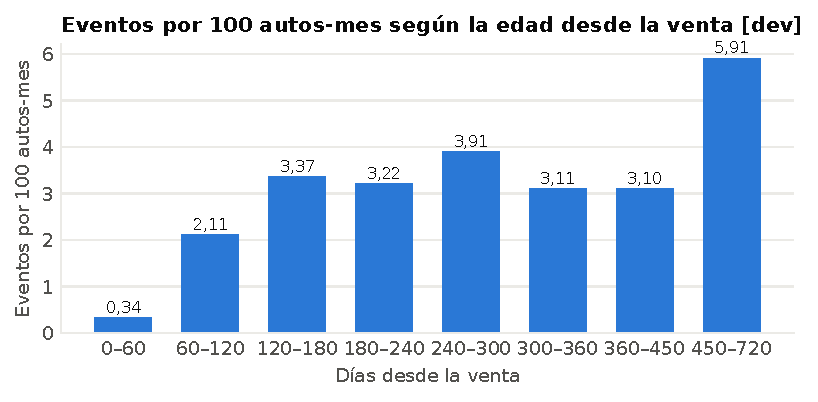
\includegraphics[width=0.9\textwidth]{figuras/riesgo_edad.pdf}
\caption{Riesgo por días desde la venta (Poisson con exposición, un registro por auto-día hasta el evento o el
fin de extracción). Sube hasta los \textasciitilde4 meses y entre los 4 y los 15 meses queda en
\textasciitilde3–4 eventos por 100 autos-mes.}
\label{fig:riesgo}
\fuente{\repo{docs/\allowbreak{}memoria/\allowbreak{}f9-eda-v2.md} §B (dev).}
\end{figure}

\textbf{El riesgo es de edad, no de kilómetros} (figura~\ref{fig:riesgo}). Ajustando por días desde la venta,
mercado y motor, el mes calendario no agrega nada (p = 0,16): no hay una ventana del registro. Lo que sí
agrega es la \emph{cohorte de venta}: los vendidos en el primer trimestre de 2025 fallan 2,1 veces más que los
del segundo a igual edad (p = 0,005). Es el mismo gradiente de producción del universo, y por eso las fechas
quedan fuera del modelo.

\begin{figure}[H]
\centering
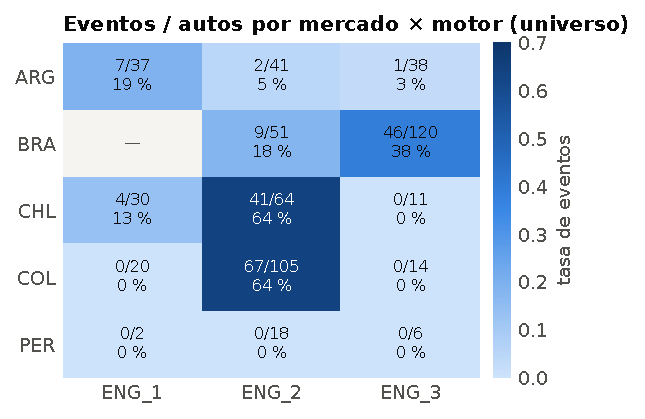
\includegraphics[width=0.62\textwidth]{figuras/celdas.pdf}
\caption{Eventos sobre autos por mercado × motor en el universo de 557. Tres celdas concentran casi todas
las fallas. Las tasas por mercado están cruzadas con cómo Ford armó la lista de fallados, así que no se leen
como física del mercado.}
\label{fig:celdas}
\fuente{\repo{docs/\allowbreak{}memoria/\allowbreak{}f9-universo-v2.md} §3.}
\end{figure}

\textbf{Dónde se concentra} (figura~\ref{fig:celdas}). En el universo, Colombia × ENG\_2 (67 de 105), Chile ×
ENG\_2 (41 de 64) y Brasil × ENG\_3 (46 de 120) concentran casi todas las fallas. Dentro de Brasil, ENG\_3 falla
2,5 veces más que ENG\_2 a igual edad, mientras que en Chile y Colombia ENG\_1 y ENG\_3 casi no fallan. Esto
define el piso más exigente del proyecto: saber mercado y motor, sin mirar un solo viaje, ya ordena muchísimo.
Qué parte de esa tasa es física (combustible, altura, motor) y qué parte es cómo se armó la lista no se puede
separar con estos datos: es la pregunta más importante para Ford.

\subsection{Consistencia y trazabilidad del pipeline}
\label{sec:trazabilidad}

\begin{itemize}
  \item \textbf{Las correcciones de los crudos se declaran, no se programan sueltas.} El loader
    (\repo{src/\allowbreak{}data/\allowbreak{}loader.py}) aplica por parte y por tabla lo que dice \repo{configs/\allowbreak{}data/\allowbreak{}raw\_sources.yaml}:
    renombres, corrimientos de origen, corte en el fin de extracción y formato de fechas. La entrega 1 se
    sigue leyendo con su propio YAML (\repo{raw\_sources\_v1.yaml}), bit a bit.
  \item \textbf{Un solo lugar por decisión.} El universo vive en \repo{src/\allowbreak{}data/\allowbreak{}usable.py}, los clones en
    \repo{configs/\allowbreak{}data/\allowbreak{}vehicle\_dedupe.yaml}, el split en \repo{src/\allowbreak{}eval/\allowbreak{}splits.py}. El recorte a desarrollo se
    hace por pertenencia explícita a la lista congelada, y el código falla si el panel trae un vehículo
    excluido (señal de que se construyó con el universo viejo).
  \item \textbf{Holdouts congelados y reproducibles.} El de la entrega 1 se reproduce bit a bit (huella
    \texttt{ba9aa4d290bc6610}); el de la v2 guarda además qué autos estaban del otro lado antes.
  \item \textbf{Contrato de datos por prefijo.} Toda columna que entra a un modelo se llama \texttt{feat\_} o
    \texttt{static\_}; lo que sirve para auditar se llama \texttt{aux\_} y el entrenamiento no lo puede ver.
    Agregar una feature es una línea de YAML.
  \item \textbf{Nada se hardcodea}: cada corrida es un YAML versionado en \repo{configs/\allowbreak{}}, y sus métricas y su
    configuración completa quedan en \repo{results/\allowbreak{}}. Los paneles y el holdout se publican como artefactos de
    Weights \& Biases, en un único proyecto compartido.
  \item \textbf{Chequeos automáticos} (\repo{scripts/\allowbreak{}check\_setup.py}, más de 200) que cubren el contrato, las
    trampas de formato y las reglas antileakage; se corren antes de cada merge.
  \item \textbf{Cada hallazgo tiene su evidencia y su comando} en \repo{docs/\allowbreak{}memoria/\allowbreak{}}, y cada decisión su fecha
    y su motivo en \repo{docs/\allowbreak{}memoria/\allowbreak{}decisiones.md}. Los comandos para reproducir este informe están en el
    Anexo~\ref{anx:repro}.
\end{itemize}

% ============================================================================ 5 · Expectativas de solución
\section{Expectativas de solución}
\label{sec:solucion}

Ford espera que la solución tenga algún aspecto de por lo menos uno de cuatro campos: análisis de datos,
inteligencia artificial, machine learning o deep learning. La nuestra usa los cuatro:
\begin{itemize}
  \item \textbf{Análisis de datos}: las auditorías de los crudos, el universo y la comparación dentro del
    mercado (§\ref{sec:datos}).
  \item \textbf{Machine learning}: modelos tabulares, de supervivencia en tiempo discreto y de cura, con
    validación agrupada y auditorías de leakage.
  \item \textbf{Deep learning}: el finalista es una red recurrente con atención sobre la secuencia de la ventana.
  \item \textbf{IA generativa}: agentes que redactan los avisos, controlados por un verificador en código.
\end{itemize}

% ---------------------------------------------------------------------------------------------- 5.1
\subsection{Objetivo de mejora: anticipar con el mayor margen posible}
\label{sec:objetivo}

\subsubsection{El recorrido: más de 40 modelos, la misma cuenta}

Probamos de lo simple a lo complejo, y cada familia nos enseñó algo. La tabla~\ref{tab:recorrido} resume el
camino. Las cifras de la entrega 1 no se comparan con las de la v2: la población, las etiquetas y el nulo
cambiaron.

\begin{table}[H]
\centering
\caption{Qué probamos, qué dio y qué aprendimos. Todo es de desarrollo salvo donde dice [test].}
\label{tab:recorrido}
\scriptsize
\begin{tabularx}{\textwidth}{@{}>{\raggedright\arraybackslash}p{3.6cm}>{\raggedright\arraybackslash}p{4.1cm}>{\raggedright\arraybackslash}X@{}}
\toprule
Modelo o idea & Resultado & Qué aprendimos \\
\midrule
\multicolumn{3}{@{}l}{\textbf{Entrega 1} (290 autos de desarrollo, 2 mercados)} \\
Logística y LightGBM sobre 53 features & PR-AUC por debajo del techo de cohorte; \aprime{} del control
  −0,0055 ± 0,0040 & Aprenden \emph{qué auto}, no \emph{cuándo}. Cambiamos la métrica (§\ref{sec:metricas}) \\
Proceso gamma de degradación & No se implementó & No hay carga irreversible medible a estos kilometrajes
  (el 51\,\% de las regeneraciones termina en 0 exacto) \\
Horizonte ordinal (bins) & No reemplaza al binario & Afinar bins no mueve la aguja \\
TimesFM zero-shot (Google) & No le gana a la tasa base & Sugirió medir el desvío respecto de la historia del
  auto; lo medimos y tampoco sumó \\
CNN-LSTM de la tutora & 11,9\,\% ± 3,6 al 5\,\% (3 repeticiones) & Con pocos eventos, las redes no tienen con
  qué aprender \\
Survival stacking (hazard por bin de km) & Único con \aprime{} positivo estable (+0,016 ± 0,003); calibrado
  (Brier 0,112) & Finalista de F3: elegido por \aprime{} y estabilidad, no por PR-AUC \\
Efecto aleatorio por auto (GPBoost) & Pierde contra el apilado simple & El efecto por auto absorbe justo lo que
  distingue autos \\
Cure model por hito post-venta & Señal real (p = 0,005) pero empata con un solo número de uso (km por día) &
  El rasgo temprano existe y es débil \\
K2: survival stacking con la ventana del registro & 17,0\,\% ± 3,8 al 5\,\%; el embolsado, 15,6\,\% &
  Finalista de la entrega 1; el pitch de entonces citaba \textasciitilde15–17\,\% \\
\midrule
\multicolumn{3}{@{}l}{\textbf{Entrega v2} (446 autos de desarrollo, 5 mercados, 135 fallados con cortes)} \\
K2 sin su ventana & Falla \aprime{}; survival stacking detecta \textasciitilde11–14\,\% al 5\,\% & La corrección de
  K2 era la ventana, que en v2 no existe \\
Re-medición de 42 modelos & GRU + viajes + estática ×3: 27 · 42 · 61\,\% al 5 · 10 · 20\,\% & Con 3× los
  eventos, los secuenciales pasan adelante; ninguno le gana con evidencia a la celda \\
Sweep bayesiano de la GRU (130 trials) & El mejor empata con semillas nuevas (0,469 contra 0,471) & La semilla
  mueve más que los hiperparámetros (0,395–0,476): se reporta un ensamble de 3 \\
GRU con etiqueta suave lejos del evento & +9,6 [3,0; 14,4] en dev; −13,3 [−25,0; +3,9] \tagtest{} & Ganaba en dev y
  no se sostuvo (§\ref{sec:suave}) \\
10 semillas y ensambles heterogéneos & Ninguno se mueve más de ±3 puntos al 5–10\,\% & Hay un techo de
  información, no de modelo \\
MiniRocket (kernels aleatorios + ridge) & 16 · 27 · 39\,\% contra 28 · 43 · 61\,\% de la GRU; −16 al 10\,\%
  [−26; −8] & Pierde con evidencia: las convoluciones aprendidas usan mejor la poca señal \\
\bottomrule
\end{tabularx}
\fuente{\repo{decisiones.md} (20-09 a 01-10); \repo{f3-mejor-modelo-a-la-fecha.md};
\repo{f9-remedicion-completa-v2.md}; \repo{f10-sweep-gru.md}; \repo{f11-*.md}; \repo{f12-preregistro-deteccion.md};
MiniRocket: \repo{origin/\allowbreak{}exp/\allowbreak{}minirocket:docs/\allowbreak{}memoria/\allowbreak{}f13-preregistro-minirocket.md}.}
\end{table}

\begin{table}[H]
\centering
\caption{Los modelos principales re-medidos sobre el dev v2 \tagdev{}: detección (\%) con umbral exacto,
promedio de 3 repeticiones; AUC por auto agrupado y dentro de mercado × motor.}
\label{tab:dev}
\small
\begin{tabular}{@{}lrrrrr@{}}
\toprule
Modelo & AUC auto & AUC celda & 5\,\% & 10\,\% & 20\,\% \\
\midrule
\textbf{GRU + viajes + estática ×3 (finalista)} & 0,82 & 0,65 & 27 & 42 & 61 \\
CNN-LSTM + viajes + estática ×3 & 0,81 & 0,62 & 22 & 41 & 62 \\
CNN-LSTM de la tutora + estática ×3 & 0,82 & 0,62 & 27 & 40 & 68 \\
Survival stacking (F3) & 0,72 & 0,57 & 14 & 24 & 42 \\
LightGBM (control, 53 features) & 0,72 & 0,57 & 18 & 28 & 42 \\
Logística L2 & 0,71 & 0,58 & 15 & 23 & 37 \\
\midrule
Celda mercado × motor (sin modelo) & 0,81 & 0,46 & 18 & 33 & 62 \\
Solo el odómetro del corte & 0,42 & 0,43 & 3 & 6 & 15 \\
Azar (puntaje permutado, historial conservado) & — & — & 5 & 11 & 21 \\
\bottomrule
\end{tabular}
\fuente{\repo{docs/\allowbreak{}memoria/\allowbreak{}f9-remedicion-completa-v2.md} (42 modelos, con la tabla completa y las comparaciones pareadas).}
\end{table}

\textbf{La lectura conjunta.} Los secuenciales ordenan autos \emph{dentro} de la celda mercado × motor con
AUC 0,62–0,65, contra 0,57 de survival stacking y de los tabulares, y le ganan a survival stacking con
evidencia entre el 10 y el 20\,\% de falsas alarmas (GRU con estática, +18,8 puntos al 10\,\%, IC95 [9,1; 27,9]).
La celda sola, en cambio, es un piso altísimo: el uso le suma \textasciitilde5–10 puntos al 5–10\,\% y al
20\,\% empata. Con la primera entrega (53 fallados) la CNN-LSTM quedaba por debajo de survival stacking: las
redes necesitaban los datos que trajo la v2.

\subsubsection{El finalista: una red que lee los viajes en orden y recuerda}
\label{sec:gru}

\begin{figure}[H]
\centering
\begin{tikzpicture}[font=\sffamily\scriptsize,
  bin/.style={draw=fordblue!60,fill=softbg,minimum width=6mm,minimum height=9mm,inner sep=0pt},
  cell/.style={draw=fordblue,fill=fordblue!15,rounded corners=2pt,minimum width=7mm,minimum height=6mm},
  blk/.style={draw=inksec,fill=white,rounded corners=2pt,align=center,inner sep=3pt},
  arr/.style={-{Stealth[length=1.6mm]},draw=inksec}]
\foreach \i/\l in {0/1,1/2,2/3,4/20} {
  \node[bin] (b\i) at (\i*1.05,0) {\l};
  \node[cell] (h\i) at (\i*1.05,1.25) {$h_{\l}$};
  \draw[arr] (b\i) -- (h\i);
}
\node at (3*1.05,0) {\dots}; \node at (3*1.05,1.25) {\dots};
\draw[arr] (h0) -- (h1); \draw[arr] (h1) -- (h2); \draw[arr] (h2) -- ++(0.6,0); \draw[arr] (3.5,1.25) -- (h4);
\node[below=1mm of b2,align=center,text width=5.2cm] {20 tramos de 50 km (los últimos 1.000 km) ×
  15 canales: cómo se viaja y qué hace el filtro};
\node[blk,above=6mm of h2,text width=3.6cm] (att) {\textbf{Atención}: un peso por tramo y el promedio pesado de
  las 20 memorias};
\foreach \i in {0,1,2,4} {\draw[arr,muted] (h\i) -- (att);}
\node[blk,left=10mm of att,text width=3cm] (st) {\textbf{País, motor y serie}\\(rama estática de 4)};
\node[blk,above=6mm of att,text width=3.6cm] (head) {\textbf{Cabeza} (16) → puntaje de riesgo a 3.000 km};
\draw[arr] (att) -- (head); \draw[arr] (st) |- (head);
\node[blk,right=6mm of head,text width=3.2cm,draw=accent2!80,fill=warnbg] (ens) {\textbf{3 redes} (semillas 42, 1, 2)
  votan por rango};
\draw[arr] (head) -- (ens);
\node[right=2mm of h4,align=left,text width=3.4cm,inksec] {GRU unidireccional, memoria de 24 números; dos
  compuertas deciden qué anotar y qué olvidar en cada tramo};
\end{tikzpicture}
\caption{La GRU finalista. Unos 3.900 parámetros: GRU 2.952, atención 416, rama estática 52 y cabeza 481.}
\label{fig:gru}
\fuente{\repo{src/\allowbreak{}models/\allowbreak{}gru\_seq.py}; \repo{configs/\allowbreak{}exp\_v2all\_gru\_trips\_estaticas\_r3.yaml};
\repo{docs/\allowbreak{}pitch/\allowbreak{}presentacion-contenido.md} (“La GRU por dentro”).}
\end{figure}

\begin{itemize}
  \item \textbf{Qué lee.} Cada 500 km, los últimos 1.000 km del auto en 20 tramos de 50 km. Cada tramo trae 15
    señales: 6 de cómo se viaja (cantidad de viajes, ralentí, viajes que no llegan a temperatura, velocidad, km
    y duración por viaje) y 9 de qué hace el filtro (registros, cobertura, acumulación media y máxima, cuánto
    sube, caídas por regeneración y tres tipos de aviso). Se imputan y estandarizan con el train de cada fold.
  \item \textbf{Cómo recuerda.} Una GRU de una capa, unidireccional, con una memoria de 24 números que se
    actualiza tramo a tramo. La \emph{compuerta de actualización} decide qué parte de la memoria se reemplaza
    con lo nuevo, y la \emph{de reinicio}, cuánto del pasado se usa para armar ese candidato. Así ve
    tendencias que un promedio de los 1.000 km borra: que el hollín viene subiendo o que los viajes se vienen
    acortando. No lee al revés: el estado en el km 200 nunca depende del km 900.
  \item \textbf{Qué mira al final.} Una capa de atención pesa los 20 tramos y arma un resumen. Se le suman país,
    motor y serie por una rama estática chica, y una cabeza da el puntaje.
  \item \textbf{Cómo aprende.} Con la etiqueta dura (1 si el evento cae entre 500 y 3.500 km después del corte),
    sobre las \textasciitilde11.700 filas de desarrollo. La pérdida pesa más los positivos (negativos sobre
    positivos del train). Adam con tasa 0,001, weight decay 1e-4, recorte del gradiente en 1,0, dropout 0,3, 40
    épocas fijas, lote de 64, en CPU. Sin early stopping: el modelo no conoce el vehículo, así que no puede
    apartar una validación agrupada propia.
  \item \textbf{Por qué chica.} Con 135 autos que fallan para aprender, una red más grande memoriza autos en vez
    de hábitos. La GRU tiene una compuerta menos que una LSTM, y por eso menos parámetros para la misma tarea.
  \item \textbf{Ensamble.} Tres redes con semillas distintas (42, 1 y 2); se promedia el rango de cada una. Las
    semillas son las del reporte v2 y no se eligieron por resultado. La alerta salta con dos cortes seguidos
    sobre el umbral.
  \item \textbf{Nadie le explicó el filtro.} La relación entre viajes cortos y hollín la encontró en los datos
    (§\ref{sec:explicabilidad}).
\end{itemize}

\subsubsection{El resultado, en autos que nunca vio}
\label{sec:test}

El test son los 111 autos del holdout. 103 tienen cortes en el panel: 32 fallaron y 71 no. Cada modelo se
entrenó con todo el desarrollo (446 autos) y se midió una vez con la misma cuenta que en dev
(\repo{scripts/\allowbreak{}eval\_test.py}).

\begin{figure}[H]
\centering
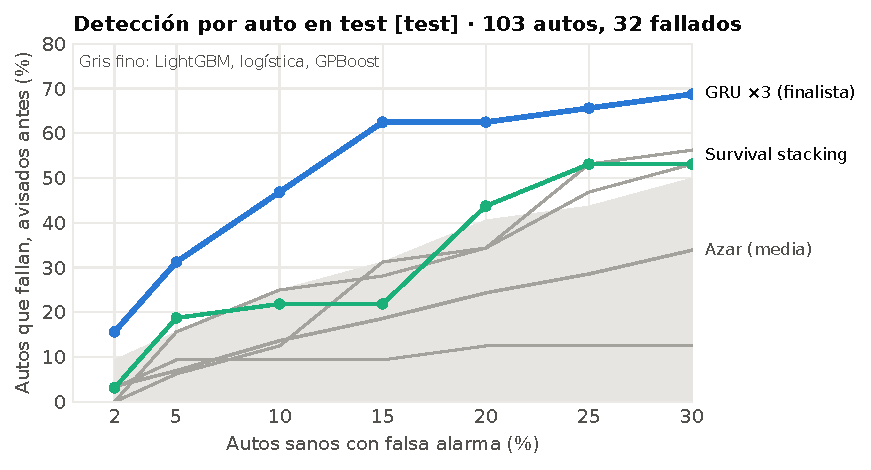
\includegraphics[width=\textwidth]{figuras/curva_test.pdf}
\caption{Detección de autos que fallan según el porcentaje de sanos con falsa alarma, en test. La banda gris
es el azar hasta su percentil 95. La celda mercado × motor no detecta nada por debajo del 10\,\% porque alerta
celdas enteras.}
\label{fig:curva}
\fuente{\repo{experiments/\allowbreak{}test-modelos-v2/\allowbreak{}curve.csv} (\repo{configs/\allowbreak{}eval\_test\_modelos\_v2.yaml}); figura:
\repo{scripts/\allowbreak{}make\_report\_figures.py}.}
\end{figure}

\begin{table}[H]
\centering
\caption{El finalista en test \tagtest{}: detección (\%) por presupuesto de falsas alarmas.}
\label{tab:test}
\small
\begin{tabular}{@{}lrrrrr@{}}
\toprule
 & 5\,\% & 10\,\% & 15\,\% & 20\,\% & Primario (5–20\,\%) \\
\midrule
\textbf{GRU ×3 (semillas 42, 1, 2)} & \textbf{31,2} & \textbf{46,9} & \textbf{62,5} & \textbf{62,5} & \textbf{50,8} \\
Survival stacking (finalista de la entrega 1) & 18,8 & 21,9 & 21,9 & 43,8 & 26,6 \\
Celda mercado × motor (sin modelo) & 0,0 & 21,9 & 21,9 & 50,0 & 23,4 \\
Azar, media & 7,0 & 13,7 & 18,6 & 24,4 & — \\
Azar, p95 & 15,6 & 25,0 & 31,2 & 40,6 & — \\
\bottomrule
\end{tabular}
\fuente{\repo{experiments/\allowbreak{}test-f10-s42/\allowbreak{}report.json}, \repo{experiments/\allowbreak{}test-modelos-v2/\allowbreak{}report.json};
\repo{docs/\allowbreak{}memoria/\allowbreak{}f11-test-resultado.md}. Todos los modelos, en el Anexo~\ref{anx:modelos}.}
\end{table}

\begin{itemize}
  \item \textbf{10 de 32 al 5\,\%: casi uno de cada tres}, 4,5 veces el azar y por encima de su p95. Al 20\,\%,
    seis de cada diez.
  \item \textbf{Le duplica el primario a los tabulares y a survival stacking} (50,8 contra 21–27). Contra survival
    stacking, +24,2 puntos, IC95 [0,8; 43,0]: el intervalo apenas no cruza el cero, y la comparación no estaba
    preregistrada.
  \item \textbf{Contra la celda mercado × motor: +27,3 puntos, IC95 [−0,8; 46,1]}, p(diferencia ≤ 0) = 0,028.
    Queda en el límite y \emph{no} lo citamos como “le gana”.
  \item \textbf{Ordena autos}: AUC por auto 0,794; dentro de mercado × motor, 0,675. Entre autos del mismo país y
    motor, el orden es moderado.
  \item \textbf{Repitió lo de dev}: en validación cruzada daba 27,4 · 42,5 · 53,3 · 60,7\,\% (primario 46,0).
\end{itemize}

\begin{table}[H]
\centering
\caption{El punto de operación con el umbral fijado en dev \tagtest{}: se elige el umbral con los sanos de
desarrollo (15 modelos de fold) y se mide en test cuántas fallas detecta y cuántas falsas alarmas produce de
verdad.}
\label{tab:operacion}
\small
\begin{tabular}{@{}lll@{}}
\toprule
Modelo & Detección (\%) al 5 · 10 · 20\,\% & Falsas alarmas reales (\%) \\
\midrule
GRU ×3 (finalista) & 20 · 34 · 57 & 5,8 · 8,9 · 18,2 \\
Survival stacking & 13 · 20 · 33 & 4,6 · 8,3 · 15,6 \\
LightGBM (53 features) & 16 · 25 · 36 & 7,5 · 10,7 · 16,9 \\
Logística L2 (53 features) & 12 · 16 · 33 & 8,8 · 11,8 · 18,3 \\
SS + efecto aleatorio (GPBoost) & 8 · 11 · 14 & 6,5 · 11,3 · 21,5 \\
\bottomrule
\end{tabular}

\fuente{\repo{experiments/\allowbreak{}test-modelos-v2/\allowbreak{}operating.csv}.}
\end{table}

\textbf{El número para operar.} En producción el umbral no se puede elegir mirando los autos que se quieren
puntuar. Fijado con los sanos de desarrollo, la GRU detecta 20 · 34 · 57\,\% al 5 · 10 · 20\,\% con
\textbf{5,8 · 8,9 · 18,2\,\% de falsas alarmas reales}: el umbral cumple su presupuesto en autos nuevos
(tabla~\ref{tab:operacion}).

\begin{caja}[title={Por qué citamos un rango y no un número}]
\small
La configuración de la GRU se leyó tres veces en test: con las semillas 42/1/2 el 27-09 (34 · 41 · 63\,\% al
5 · 10 · 20\,\%), con las semillas 101–103 como referencia del tiro de F11 (28 · 50 · 50\,\%), y con 42/1/2 el
01-10 (31 · 47 · 63\,\%). La primera lectura fue antes del preregistro de F11 y no pudo inflar ese resultado,
pero el test ya se había mirado. Además, la GRU no es reproducible bit a bit entre corridas, aun con la misma
semilla (correlación 0,88–0,91 entre los puntajes de dos corridas con la misma configuración). Con 32 fallas,
cada auto mueve 3 puntos. Por eso: \textbf{\textasciitilde30\,\% al 5\,\%, \textasciitilde40–50\,\% al 10\,\% y
\textasciitilde50–60\,\% al 20\,\%.}

\textbf{Sin los 36 autos de test que estaban en el desarrollo de la entrega 1} (71 autos, 22 fallados): 36,4 ·
50,0 · 50,0 · 59,1\,\% al 5 · 10 · 15 · 20\,\% (primario 48,9). Lo aprendido mirando la entrega 1 no está
inflando el test.
\fuente{\repo{docs/\allowbreak{}memoria/\allowbreak{}f11-test-resultado.md} §2 y resumen.}
\end{caja}

\subsubsection{Cuánto antes: el margen medido}
\label{sec:anticipacion}

Este es el objetivo de mejora de la sección 5.1 del desafío: anticipar con la mayor cantidad de tiempo o
kilometraje posible.

\begin{itemize}
  \item \textbf{Al 10\,\% de falsas alarmas} \tagtest{}, la primera alerta llega con una mediana de
    \textbf{4.646 km} (p25–p75: 2.403–9.263 km) antes del evento, y unos \textbf{99 días} aproximados con los km
    por día de cada auto. Al 5\,\%: 3.987 km, \textasciitilde72 días. Al 20\,\%: 5.969 km, \textasciitilde109 días.
  \item \textbf{En dev} \tagdev{}, al 10\,\%: mediana \textasciitilde7.600 km (p25–p75: 3.700–13.100), \textasciitilde86
    días. En km el test da menos porque sus autos detectados andan menos km por día; en días es parecido.
    Sin los autos vistos en la entrega 1, la mediana en test es de \textasciitilde8.800 km.
  \item \textbf{El piso es el gap}: por construcción, ninguna alerta usa los 500 km previos al evento. La distancia
    se mide hasta la referencia del evento (fecha registrada − 21 días); hasta la fecha registrada, el margen es
    algo mayor.
\end{itemize}

\begin{figure}[H]
\centering
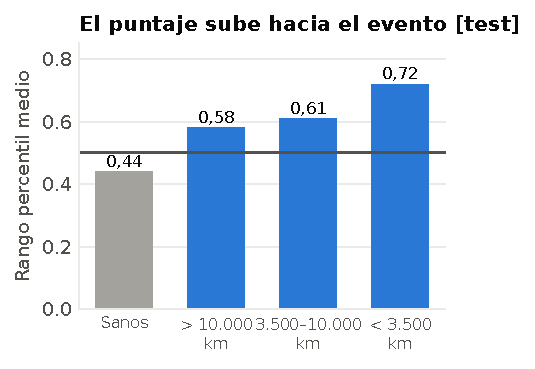
\includegraphics[width=0.62\textwidth]{figuras/score_evento.pdf}
\caption{Rango percentil medio del puntaje en los cortes de autos que fallan, según la distancia al evento, y en
los sanos. El fallado ya está por encima de los sanos lejos del evento (\emph{qué auto}) y sube al acercarse
(algo de \emph{cuándo}).}
\label{fig:score}
\fuente{\repo{docs/\allowbreak{}memoria/\allowbreak{}f11-test-resultado.md} §4 (test, promedio de las 3 semillas).}
\end{figure}

\textbf{Cómo se lee el margen.} El puntaje sube a medida que se acerca el evento (figura~\ref{fig:score}), y la
primera alerta cae a mitad del historial, no en el primer corte: hay algo de \emph{cuándo}. Pero la dispersión es
enorme, y la auditoría \aprime{} del finalista da +0,001 (§\ref{sec:limites}). Por eso la frase defendible es
“\emph{lo marcamos con unos tres meses de margen}”, nunca “\emph{predecimos que falla en tres meses}”.

\subsubsection{Una variante que ganaba en desarrollo y no se sostuvo}
\label{sec:suave}

Es el aprendizaje metodológico más importante del proyecto. Con la etiqueta dura, un corte a 10.000 km del
evento de un auto que falla se entrena igual que uno de un auto sano, aunque la detección se cuente por auto. La
variante F11 entrenaba esos cortes lejanos con 0,15 en vez de 0 (una etiqueta suave).

\begin{itemize}
  \item \textbf{En desarrollo ganaba con evidencia}, en una confirmación preregistrada con folds y semillas
    nuevos: +9,6 puntos de primario, IC95 [3,0; 14,4], p = 0,0015 (34,6 · 48,6 · 60,2 · 70,1\,\% al 5 · 10 · 15 ·
    20\,\%). Era el primer modelo que le ganaba con evidencia a la celda.
  \item \textbf{En el tiro preregistrado en test no se sostuvo}: 31,2 contra 44,5 de la GRU con la etiqueta dura,
    −13,3 puntos, IC95 [−25,0; +3,9]. La regla escrita antes decía “no se sostiene”, y así se reportó, sin buscar
    variantes.
  \item \textbf{Por qué}: en test se comportó como la tasa de la celda (al 10 y al 20\,\% detecta exactamente lo
    mismo que la celda sola) y perdió el orden dentro de la celda (AUC 0,689 en dev, 0,571 en test). El 0,15 en
    todos los cortes lejanos premiaba reconocer a \emph{ese auto} en cualquier momento, y lo más estable de un
    auto es su país, su motor y su serie.
  \item \textbf{Lo que nos llevamos}: la confirmación usó folds y semillas nuevos, pero los mismos 446 autos sobre
    los que se habían explorado unas 20 variantes. Un holdout que nadie toca es lo único que separa una mejora
    real del optimismo de desarrollo. El finalista es la GRU con la etiqueta dura porque era la referencia
    preregistrada y el candidato no se sostuvo, no porque se haya elegido entre varios modelos mirando test.
\end{itemize}

\subsubsection{Límites}
\label{sec:limites}

\begin{limite}[title={Lo que el modelo no puede afirmar}]
\small
\begin{enumerate}
  \item \textbf{No le gana con evidencia a la celda mercado × motor} \tagtest{} (+27,3, IC95 [−0,8; 46,1]). Parte
    de lo que detecta es composición: el país pesa (§\ref{sec:explicabilidad}).
  \item \textbf{Sabe poco del cuándo}: \aprime{} = +0,001 \tagdev{} (colapsar el puntaje al promedio del auto casi no
    cambia nada). Es positivo, como en todos los modelos de la v2, pero chico.
  \item \textbf{Con 32 fallas, los intervalos son anchos}, y el orden entre familias tampoco es firme: sin los
    autos vistos, LightGBM y survival stacking suben a \textasciitilde50 de primario y empatan con la GRU
    (survival stacking − GRU: +1,1, IC95 [−20,5; +27,3]).
  \item \textbf{El test se leyó más de una vez}: se cita un rango. Ninguna variante nueva se mide contra él;
    una mejora sobre este modelo necesita datos nuevos.
  \item \textbf{La muestra está enriquecida en fallas} (135 de 426 autos de desarrollo con cortes; 32 de 103 en
    test). Los conteos de alertas no se trasladan a una flota real, y el puntaje ordena autos: no es una
    probabilidad calibrada a la prevalencia real.
  \item \textbf{No predecimos la fecha exacta}: marcamos con margen, con una dispersión grande.
  \item \textbf{La referencia del evento corrida 21 días es poblacional}: no se puede fechar la intervención auto
    por auto.
\end{enumerate}
\end{limite}

% ---------------------------------------------------------------------------------------------- 5.2
\subsection{Criterios de evaluación}
\label{sec:criterios}

\subsubsection{Viabilidad técnica}
\label{sec:viabilidad}

\textbf{Lo que ya existe y funciona.}
\begin{itemize}
  \item \textbf{Un modelo medido en autos que nunca vio}, con su umbral de operación fijado fuera de muestra y
    cumpliendo el presupuesto de falsas alarmas (§\ref{sec:test}).
  \item \textbf{Un pipeline reproducible} de punta a punta, desde los seis CSV hasta el puntaje, con las
    correcciones declaradas y más de 200 chequeos automáticos (§\ref{sec:trazabilidad}).
  \item \textbf{Una demo de producto} desplegada (§\ref{sec:producto}) que reproduce la flota de desarrollo semana a
    semana.
\end{itemize}

\textbf{Por qué escala sin hardware nuevo.}
\begin{itemize}
  \item \textbf{Cero sensores nuevos}: solo resúmenes por viaje y mensajes del filtro que el auto conectado ya
    manda.
  \item \textbf{Modelo liviano}: \textasciitilde3.900 parámetros, en CPU, sin GPU ni para servir ni para
    reentrenar. Hoy las 56 corridas de la re-medición completa tardaron \textasciitilde25 minutos en 24 núcleos.
  \item \textbf{El mismo código de features en entrenamiento y en producción} (\repo{src/\allowbreak{}features},
    \repo{src/\allowbreak{}data/\allowbreak{}panel.py}). Si producción reimplementara las features, los números del piloto dejarían de ser
    los medidos.
  \item \textbf{Los agentes trabajan solo sobre las alertas}, no sobre la flota: el costo de IA crece con los
    avisos, no con los autos.
\end{itemize}

Para un millón de autos con \textasciitilde3 viajes por día, estimamos un batch diario de 1–2 horas en 8–16 vCPU
(\textasciitilde3 millones de filas de viajes por día). Es una estimación propia que hay que validar con el equipo
de datos de Ford.

\begin{table}[H]
\centering
\caption{Cómo llega a producción.}
\label{tab:etapas}
\scriptsize
\begin{tabularx}{\textwidth}{@{}>{\raggedright\arraybackslash}p{2.4cm}>{\raggedright\arraybackslash}X>{\raggedright\arraybackslash}p{1.6cm}>{\raggedright\arraybackslash}p{4cm}@{}}
\toprule
Etapa & Qué & Duración & Criterio para pasar \\
\midrule
0 · Congelar & Reentrenar con los 557 autos y empaquetar el modelo (pesos por semilla, export ONNX, referencia del
  ensamble, umbrales, 20 autos de control) & 1–2 semanas & El paquete re-puntúa los autos de control igual \\
1 · Piloto en sombra & Puntuar la flota real de un mercado (Colombia o Chile, los de más eventos) sin avisar a nadie
  & 3–6 meses & Tasa de alertas ≈ presupuesto elegido; detección realizada ≥ celda mercado × motor \\
2 · Piloto activo & Avisos en una región, con un grupo control sin aviso & 6 meses & Fallas evitadas contra el
  control; costo por alerta; cambio de hábitos \\
3 · Escala & Todos los mercados validados, umbral recalibrado por mercado & continuo & Monitoreo en verde \\
\bottomrule
\end{tabularx}
\fuente{\repo{docs/\allowbreak{}pitch/\allowbreak{}presentacion-contenido.md} bloque 5.}
\end{table}

\textbf{Por qué la sombra es el paso clave.} Todo lo que medimos salió de las listas que Ford armó para el desafío,
muestreadas en dos cohortes. La sombra es la primera medición de la prevalencia real por mercado × motor y de las
falsas alarmas sobre la flota completa. También responde la duda más grande del proyecto: qué parte de lo que el
modelo aprende es física y qué parte es cómo se armaron las listas.

\textbf{Monitoreo y reentrenamiento.} Tasa de alertas por mercado contra el presupuesto; deriva de las features
por mercado y mes; detección realizada (cada falla en taller, ¿tuvo alerta antes y con cuánto margen?); datos que
dejan de llegar (ya pasó con el contador de regeneraciones); rechazos del verificador. Reentrenamiento trimestral
o con +50\,\% de eventos nuevos, con las mismas auditorías y comparado en sombra contra el modelo vigente.

\textbf{Lo que falta escribir}: hoy el entrenamiento guarda predicciones, no modelos; el empaquetado
(\repo{export\_model.py}) está diseñado pero no implementado. No toca nada de lo medido.

\paragraph{El producto, funcionando: la demo.}
\label{sec:producto}

La demo (Streamlit, desplegada con clave) reproduce semana a semana los 426 autos de desarrollo con cortes (135
que fallan y 291 sanos), del 03-03-2025 al 24-09-2026, con el modelo finalista tal cual. El test no se muestra
nunca: el bundle falla si aparece un auto de test. Tiene tres pantallas:
\begin{itemize}
  \item \textbf{Bandeja} (el gerente de posventa, cada lunes): una tarjeta por alerta con el mensaje al conductor,
    el resumen del taller y los hechos en los que se apoya cada texto, con el tilde del verificador.
  \item \textbf{Vehículo} (el concesionario): el puntaje contra el umbral, la alerta y los hábitos en los que el
    auto se aparta de los sanos de su mercado.
  \item \textbf{Qué pasó después}: el replay al lado de los números oficiales.
\end{itemize}
Una \textbf{perilla} arriba de cada pantalla elige el punto de operación (5, 10, 15 o 20\,\% de sanos con un aviso
de más) y mueve todo lo demás.

\begin{table}[H]
\centering
\caption{La demo por punto de la perilla \tagdev{}. El replay es una repetición de la CV; los oficiales, el
promedio de tres.}
\label{tab:demo}
\scriptsize
\begin{tabular}{@{}lrrrr@{}}
\toprule
 & 5\,\% & 10\,\% & 15\,\% & 20\,\% \\
\midrule
Detección oficial (3 repeticiones) & 28,1 & 42,5 & 53,1 & 61,0 \\
Fuera de muestra: detección / falsas alarmas reales (\%) & 27,9 / 4,9 & 42,5 / 10,2 & 52,3 / 15,1 & 60,7 / 19,9 \\
Azar, media (mismo historial) & 5,4 & 10,7 & 15,7 & 20,7 \\
Replay: fallas avisadas antes (de 135) & 39 & 56 & 69 & 82 \\
Replay: sanos con un aviso de más (de 291) & 14 & 29 & 43 & 58 \\
Replay: alertas / escalamientos & 53 / 7 & 85 / 10 & 112 / 22 & 140 / 36 \\
Replay: alertas con un hábito para nombrar & 48 & 73 & 101 & 125 \\
Replay: anticipación mediana, alerta → falla (semanas) & 15 & 16 & 16 & 21 \\
Replay: ídem, en km & 7.000 & 7.200 & 7.500 & 8.100 \\
\bottomrule
\end{tabular}
\fuente{\repo{feat/\allowbreak{}demo-gru:docs/\allowbreak{}memoria/\allowbreak{}f9-demo-gru-final.md}; bundle \repo{experiments/\allowbreak{}demo-bundle-gru-final}.}
\end{table}

\textbf{Los agentes y el verificador.} Dos agentes (\texttt{gpt-5.4-mini}): el \emph{redactor} escribe el mensaje
al conductor, el resumen para el taller y la línea de la bandeja, eligiendo recomendaciones de listas cerradas;
el de \emph{triage} recorre los eventos de la semana con herramientas, pide la acción a la política (no puede
elegir otra) y arma el resumen semanal. El \emph{verificador}, en código, rechaza todo número que no esté en los
hechos, el lenguaje causal (“porque”, “debido a”), las certezas, las promesas de que el riesgo baja, la palabra
“probabilidad”, los síntomas del filtro en un texto al conductor y la atribución (“el sistema lo marcó por…”). Si
rechaza, el agente reintenta hasta dos veces; si no lo logra, queda una plantilla aprobada. En la temporada
completa, con los cuatro puntos de la perilla, los agentes redactaron \textbf{465 textos y 196 resúmenes}, todos
aprobados por el verificador, con 40 intentos rechazados en el camino y ninguna plantilla. Cada respuesta queda
en una caché por el hash de lo que la define, así que la demo se reproduce sin red.

\subsubsection{Costo}
\label{sec:costo}

\textbf{Lo que cuesta operar el producto.} Estimación propia para un millón de autos conectados, a validar con
Ford (tabla~\ref{tab:costo}). El 80\,\% del costo anual es la persona que lo opera: agregar autos casi no lo mueve.
El costo real no es la computadora, sino integrar el sistema con Ford (ingesta, app, concesionarios) y el costo
de cada alerta.

\begin{table}[H]
\centering
\caption{Costo anual de operación para 1 millón de autos (estimación propia).}
\label{tab:costo}
\small
\begin{tabular}{@{}lrl@{}}
\toprule
Componente & USD por año & Supuesto \\
\midrule
Features + puntaje diario & 2.500–6.000 & batch de 1–2 h en 8–16 vCPU \\
Agentes (LLM) & 1.000–3.000 & \textasciitilde65.000 alertas por año × \textasciitilde6 llamadas, modelo chico \\
Reentrenamiento + monitoreo & 5.000–10.000 & trimestral, en CPU \\
Equipo de operación & 60.000–80.000 & 1 persona de ML/MLOps \\
\midrule
\textbf{Total} & \textbf{\textasciitilde70.000–100.000} & \textbf{\textasciitilde USD 0,07–0,10 por auto y por año} \\
\bottomrule
\end{tabular}
\fuente{\repo{docs/\allowbreak{}pitch/\allowbreak{}presentacion-contenido.md} bloque 6. Implementación, una sola vez:
\textasciitilde USD 70.000–110.000 (tres personas durante 6 meses, incluye la sombra).}
\end{table}

\textbf{Lo que no citamos: el costo de una falla.} No conocemos lo que le cuesta a Ford. Con la primera entrega
armamos escenarios con precios públicos de EE.\,UU. (diagnóstico USD 100–250, falla USD 800–15.000) sobre el
finalista de entonces (\repo{f8-costos-k2.md}). Lo que dejaron es una forma de pensar, no un ahorro:
\begin{itemize}
  \item si la falla es barata, lo óptimo es no alertar; si la alerta es casi gratis, alertar a todos le gana a
    cualquier modelo;
  \item el modelo paga en una franja: cuando el beneficio de anticipar es de \textasciitilde5 a \textasciitilde15
    veces el costo de una inspección y la prevalencia real es de 2–5\,\%;
  \item por eso pedimos a Ford dos números: cuánto le cuesta una falla contra un diagnóstico, y la prevalencia real.
\end{itemize}

\textbf{Por qué el diseño baja el costo de equivocarse.} El primer contacto es un consejo de manejo, no un turno:
al 5\,\%, 48 de las 53 alertas del replay llevan un hábito para nombrar \tagdev{}. Si el auto no iba a fallar, el
conductor recibió un consejo que igual le hace bien al motor. Pero en una flota real la mayoría de los avisos van a
ir a autos que no iban a fallar, porque la prevalencia es mucho más baja que en la muestra:

\begin{table}[H]
\centering
\caption{Cuenta ilustrativa por cada 1.000 autos, con la detección de test (31\,\% al 5\,\%, 62\,\% al 20\,\%).}
\label{tab:prevalencia}
\small
\begin{tabular}{@{}rrrr>{\raggedright\arraybackslash}p{4.2cm}@{}}
\toprule
Prevalencia supuesta & Perilla & Fallas avisadas & Consejos de más & De cada 10 avisos, cuántos son de un auto que iba a fallar \\
\midrule
2\,\% & 5\,\% & 6 de 20 & 49 & \textasciitilde1 \\
5\,\% & 5\,\% & 16 de 50 & 48 & \textasciitilde2 \\
10\,\% & 5\,\% & 31 de 100 & 45 & \textasciitilde4 \\
5\,\% & 20\,\% & 31 de 50 & 190 & \textasciitilde1 \\
\bottomrule
\end{tabular}
\fuente{\repo{docs/\allowbreak{}pitch/\allowbreak{}presentacion-contenido.md} bloque 6 (respaldo).}
\end{table}

Es un argumento a favor del diseño: si el aviso de más fuera un turno en el taller, la fricción sería
inaceptable. Y mandarle el mismo consejo a toda la flota no sirve, porque un aviso genérico se ignora: el nuestro
dice algo cierto de ese auto (“comparado con los sanos de tu zona”). Con estos datos no pudimos medir la pérdida de
consumo (el nivel de combustible solo permite estimarla en una parte de los viajes y no separa fallados de sanos):
es la primera métrica del piloto.

\subsubsection{Carácter innovador}
\label{sec:innovacion}

\begin{enumerate}
  \item \textbf{Una métrica que no se deja engañar.} Mostramos que en este problema el PR-AUC por fila se alcanza
    sin anticipar nada (el techo de cohorte), y lo reemplazamos por la detección por auto con un presupuesto de
    falsas alarmas, contra un nulo que conserva el largo del historial y contra la regla “país × motor”. Es la
    diferencia entre un modelo que reconoce autos y uno que avisa a tiempo.
  \item \textbf{Una red que lee la ventana en orden.} La GRU con atención sobre tramos de km ve tendencias dentro
    de los 1.000 km que un agregado borra, y le duplica la detección a los modelos tabulares en test.
  \item \textbf{IA generativa con barandas.} El modelo decide, el agente comunica y el código verifica. El LLM
    nunca produce un número, un puntaje ni un diagnóstico; un verificador rechaza lenguaje causal, certezas y
    números que no estén en los hechos.
  \item \textbf{El porqué contado como comparación, no como causa.} Al conductor se le nombran solo hábitos que
    puede cambiar, en los que su auto se aparta de los sanos de su mercado y que coinciden con la física del DPF.
  \item \textbf{La perilla.} Ford elige cuántas falsas alarmas tolera según lo que le cuesta cada una, con el
    umbral fijado fuera de muestra.
  \item \textbf{Rigor como producto.} Preregistros escritos antes de medir, auditorías obligatorias y un holdout
    que se abrió una sola vez para elegir. La confianza que le pedimos al jurado es la misma que el producto
    construye con el cliente.
\end{enumerate}

\subsubsection{Calidad del tratamiento de datos}
\label{sec:calidad}

Está desarrollado en §\ref{sec:datos}. En resumen:
\begin{itemize}
  \item \textbf{Limpieza y preparación}: cinco trampas de formato de la entrega v2 corregidas al leer; 13 clones
    colapsados; fechas en dos formatos; universo simétrico por período de producción (§\ref{sec:trampas},
    §\ref{sec:universo}).
  \item \textbf{Faltantes y atípicos}: topes físicos y no cuantiles; ralentí separado de los viajes; faltantes
    estructurales tratados como información; el contador cortado, reconstruido desde el nivel del filtro
    (§\ref{sec:limpieza}).
  \item \textbf{Consistencia y trazabilidad}: correcciones declaradas en YAML, holdouts congelados con huella,
    contrato por prefijo, chequeos automáticos, cada hallazgo con su comando (§\ref{sec:trazabilidad},
    Anexos~\ref{anx:repro} y~\ref{anx:auditorias}).
\end{itemize}

\subsubsection{Claridad para mostrar los datos}
\label{sec:claridad}

\begin{itemize}
  \item \textbf{En este informe}, una figura o tabla por idea y siempre con su fuente: la curva de detección contra
    falsas alarmas con el azar dibujado (figura~\ref{fig:curva}), el perfil alineado al evento
    (figura~\ref{fig:perfil}), el riesgo por edad (figura~\ref{fig:riesgo}), las celdas mercado × motor
    (figura~\ref{fig:celdas}), el puntaje hacia el evento (figura~\ref{fig:score}) y en qué se apoya el modelo
    (figura~\ref{fig:permutacion}). Las figuras salen de un script con su YAML, desde las salidas de las corridas.
  \item \textbf{La demo de producto} (§\ref{sec:producto}): calendario de la flota con una columna por semana, la
    ficha del auto con su puntaje contra el umbral y los hábitos contra la flota sana, y la perilla. Se revisó
    visualmente en notebook y en celular.
  \item \textbf{Dashboards internos}: el del análisis exploratorio (\repo{scripts/\allowbreak{}dashboard\_eda.py}, solo
    desarrollo) y el de explicabilidad y costos del finalista de la entrega 1 (\repo{scripts/\allowbreak{}dashboard\_k2/\allowbreak{}}).
  \item \textbf{La regla de presentación}: toda detección al lado del azar; “31\,\%” solo no dice nada, “31\,\% donde
    el azar da 7\,\%” sí.
\end{itemize}

\subsubsection{Explicabilidad del modelo}
\label{sec:explicabilidad}

Explicamos en dos niveles, y no los mezclamos.

\textbf{1 · En qué se apoya la GRU} (para Ford y el equipo técnico). Permutamos cada señal (sus 20 tramos juntos)
o cada estática en la validación de cada fold y medimos cuánto cae la detección media al 5–20\,\%
(figura~\ref{fig:permutacion}).

\begin{figure}[H]
\centering
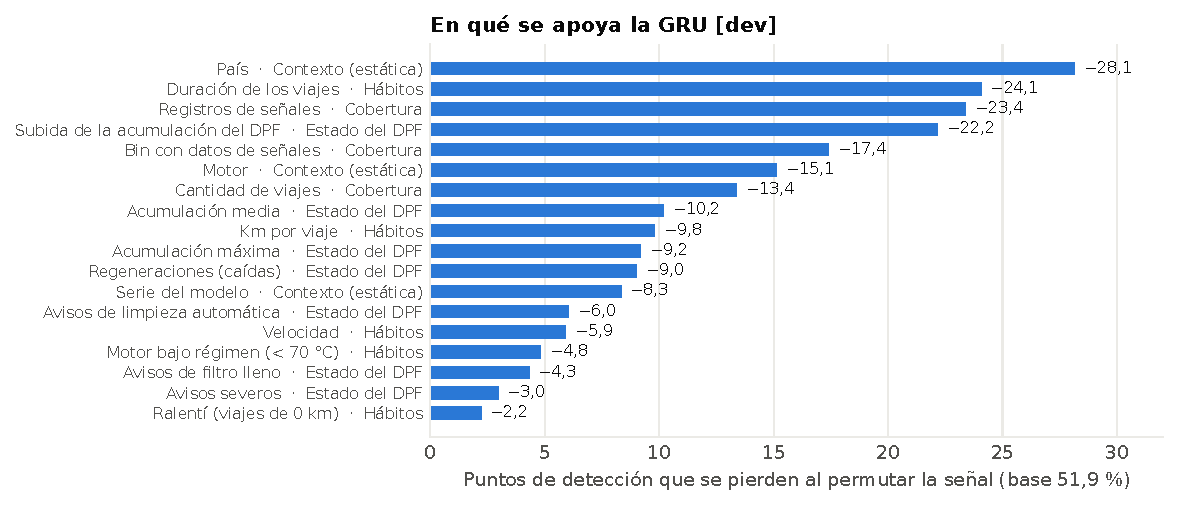
\includegraphics[width=\textwidth]{figuras/permutacion.pdf}
\caption{Caída de la detección media al 5–20\,\% al permutar cada señal en la validación (dev, semilla 42,
repetición 0; detección base 51,9\,\%). Las caídas no se suman por familia: permutar una señal sola no es
esconder la familia.}
\label{fig:permutacion}
\fuente{\repo{experiments/\allowbreak{}explain-gru-final/\allowbreak{}units.csv}; \repo{configs/\allowbreak{}explain\_gru\_final.yaml}
(\repo{scripts/\allowbreak{}explain\_perm\_seq.py}).}
\end{figure}

\begin{itemize}
  \item \textbf{Hábitos}: la duración de los viajes es el que más pesa (−24,1 puntos), por delante de km por viaje
    (−9,8), velocidad (−5,9), motor bajo régimen (−4,8) y ralentí (−2,2).
  \item \textbf{Estado del filtro}: cuánto sube la acumulación (−22,2), su nivel medio (−10,2) y máximo (−9,2), y
    las regeneraciones (−9,0).
  \item \textbf{Contexto}: el país pesa más que cualquier señal (−28,1), y el motor −15,1. Es coherente con la celda
    como piso: el riesgo no es el mismo en todos los mercados.
  \item \textbf{Cobertura}: cuántos registros y viajes hay en cada tramo (−23,4 y −13,4). Que un tramo tenga datos
    o no también informa.
\end{itemize}
La lectura física es la del DPF: viajes cortos que no dejan terminar la regeneración y hollín que se acumula. No le
dimos ninguna regla del filtro: esa relación la aprendió de los datos.

\textbf{2 · Por qué este auto} (para el conductor y el concesionario). La GRU no tiene atribución por auto, y 7 de
sus 15 canales son el estado del propio filtro, que no es algo que el conductor pueda cambiar. Por eso el porqué
que se comunica \emph{no} es lo que usó el modelo, sino una comparación descriptiva:
\begin{itemize}
  \item el promedio de los cortes que dispararon la alerta se compara con la mediana de los autos sanos de
    desarrollo del mismo mercado;
  \item un hábito “se aparta” si supera al 75\,\% de esos sanos hacia el lado riesgoso, y se nombran hasta tres;
  \item \textbf{solo se nombran hábitos accionables cuyo efecto esperado coincide con la física del DPF}, de una
    lista cerrada antes de mirar los datos. Síntomas (nivel del filtro, regeneraciones, avisos, aceite, consumo) y
    contexto (mercado, odómetro) nunca llegan al conductor: van al taller.
\end{itemize}

El criterio físico viene de la explicabilidad del finalista de la entrega 1 (SHAP sobre survival stacking,
reconstruido bit a bit): 10 de los 15 hábitos accionables con hipótesis física coincidían con la física del DPF;
cuatro iban al revés (por ejemplo, viajes más largos asociados a más riesgo) y quedaron fuera del texto al cliente
(\repo{f4-explicabilidad-k2.md}). Por eso el texto dice “comparado con autos sanos de tu zona”, nunca “porque”: el
verificador rechaza el lenguaje causal.

\subsubsection{El pitch}
\label{sec:pitch}

El pitch cuenta la misma historia que este informe, en siete bloques y 29 minutos, y con los mismos números
(tabla~\ref{tab:pitch}). El hilo es un usuario común, “nuestro conductor”: hace viajes cortos en la ciudad, su
filtro se tapa sin que nadie lo note, y al final de la historia recibe el aviso a tiempo.

\begin{table}[H]
\centering
\caption{La estructura del pitch.}
\label{tab:pitch}
\scriptsize
\begin{tabularx}{\textwidth}{@{}>{\raggedright\arraybackslash}p{2.6cm}>{\raggedright\arraybackslash}X>{\raggedright\arraybackslash}p{4.8cm}@{}}
\toprule
Bloque & Pregunta que responde & Frase ancla \\
\midrule
1 · El problema & ¿Por qué le importa a Ford? & “El auto avisa cuando el filtro ya no da más. Y el cliente se entera solo.” \\
2 · Los datos & ¿Qué hay en la telemetría y qué trampas tenía? & “La forma de manejar deja huella meses antes.” \\
3 · El modelo & ¿Qué probamos, qué ganó y cuánto detecta? & “Casi 1 de cada 3, tres meses antes, con 5\,\% de falsas alarmas.” \\
4 · El producto & ¿Qué pasa después de la alerta? (agentes y demo en vivo) & “El modelo decide. El agente habla como una persona. El código cuida lo que dice.” \\
5 · Escalabilidad & ¿Cómo llega a un millón de autos? & “Un millón de autos, sin un sensor nuevo.” \\
6 · Costos & ¿Qué pierde el cliente hoy y cuánto cuesta evitarlo? & “Cada aviso a tiempo es un cliente que confía más en Ford.” \\
7 · Cierre & ¿Por qué es distinto y qué necesita de Ford? & “Del testigo en el tablero al aviso a tiempo.” \\
\bottomrule
\end{tabularx}
\fuente{\repo{docs/\allowbreak{}pitch/\allowbreak{}presentacion-contenido.md}; deck en \repo{docs/\allowbreak{}pitch/\allowbreak{}deck/\allowbreak{}index.html}.}
\end{table}

Las reglas para citar números son las mismas en el deck y acá: toda detección al lado del azar; el resultado en test
y en rango; [test] y [dev] marcados; la anticipación como margen y no como pronóstico; nada de accuracy; y los
límites dichos antes de que los pregunten.

% ============================================================================ 6 · Información complementaria + conclusión
\section{Información complementaria}
\label{sec:complementaria}

\textbf{Documentación utilizada.} El conjunto de datos y su diccionario se recibieron en dos entregas, y el diccionario se
contrastó con los archivos columna por columna (\S\ref{sec:datos}). Cada hallazgo, decisión y experimento quedó documentado
con su fecha, su motivo y el procedimiento que lo reproduce, y cada experimento está definido por un archivo de configuración
versionado.

\textbf{Información que solo Ford puede aportar.} El límite actual no es el modelo sino la información disponible:
\begin{enumerate}
  \item \textbf{La tasa real de eventos} en la flota, que permite separar la física del criterio con que se extrajeron las
    listas. Es la principal incertidumbre del trabajo.
  \item \textbf{El origen de los 278 vehículos con evento y fecha por defecto} que salieron entre entregas, y el criterio
    de armado de la lista de vehículos con evento.
  \item \textbf{Qué registra la fecha del evento}: hoy se corre 21 días porque cae unas dos semanas después del taller.
  \item \textbf{Más eventos registrados} (hoy son 177), \textbf{la zona de uso} del vehículo (no la de venta) y \textbf{los
    costos reales} de una falla y de una inspección.
  \item \textbf{Un piloto en sombra de tres meses en un país}, para medir prevalencia, falsas alarmas y detección reales.
\end{enumerate}

\textbf{Trabajo futuro.} Reentrenar con los 557 vehículos y empaquetar el modelo. Validar toda mejora con datos nuevos (una
extracción posterior al 14-09-2026) y no con este conjunto de prueba, que ya fue utilizado. Medir en el piloto lo que estos
datos no permiten: si los avisos cambian hábitos, cuántas fallas se evitan y cuánto combustible se ahorra. Extender el
circuito a otras fallas del sistema de postratamiento.

% ============================================================================ Conclusión
\section{Conclusión}
\label{sec:conclusion}

Se mostró que la telemetría que Ford ya recibe contiene información que anticipa la saturación del filtro de partículas, y
que esa información es consistente con la física de la regeneración: los vehículos que fallan pasan más tiempo detenidos con
el motor en marcha y con el motor por debajo de su temperatura de régimen, y la diferencia crece hacia el evento. Se mostró
también que los datos contenían sesgos de muestreo y de formato capaces de producir métricas favorables sin ninguna
capacidad predictiva, y que el PR-AUC por fila tiene un piso de $0{,}177$ alcanzable sin información temporal. Por eso el
modelo se seleccionó con la detección por vehículo a presupuesto de falsas alarmas, comparada con un nulo que conserva el
historial.

Con ese criterio, el modelo finalista, una GRU con atención de $\sim 3.900$ parámetros en un ensamble de tres semillas,
detecta en vehículos no vistos $\sim 30\,\%$ de los eventos con $5\,\%$ de falsas alarmas y $\sim 50$--$60\,\%$ con $20\,\%$,
con una mediana de $\sim 4.600$\,km (unos tres meses) de anticipación y un umbral que respeta su presupuesto fuera de
muestra. Duplica la detección de los modelos tabulares y de supervivencia en el mismo conjunto. El circuito propuesto
convierte cada alerta en un aviso verificable, con el punto de operación como decisión de Ford, a un costo estimado de
USD~$0{,}07$--$0{,}10$ por vehículo y por año. La validación de su impacto sobre fallas evitadas requiere el piloto en sombra
propuesto.

\appendix
% ============================================================================ 7 · Anexos
\section{Reproducibilidad: comandos y configuraciones}
\label{anx:repro}

Todo corre desde la raíz del repositorio con el entorno de \repo{requirements.txt} (más
\repo{requirements-dl.txt} para las redes). Los datos no se versionan: la entrega v2 va en
\repo{data/\allowbreak{}v2/\allowbreak{}raw/\allowbreak{}} y se apunta con \repo{FORD\_DATA\_DIR}. Sin red, \repo{WANDB\_MODE=disabled}. Cada número de
este informe sale de alguna de estas líneas. La GRU no es reproducible bit a bit entre plataformas ni cantidades de
hilos: una reproducción da números cercanos, no idénticos.

\subsection*{Datos, universo y panel}
\begin{lstlisting}
export FORD_DATA_DIR=$PWD/data/v2 WANDB_MODE=disabled OMP_NUM_THREADS=1
# entrega 1 vs v2
python scripts/compare_deliveries.py --config configs/data/compare_deliveries.yaml
# universo + holdout
python scripts/make_test_split.py --config configs/data/test_split.yaml --force
# cache del EDA (solo dev)
python scripts/build_eda_cache.py --config configs/data/eda_cache_v2.yaml
# EDA dentro del mercado
python scripts/eda_v2.py --config configs/eda_v2.yaml
# panel agregado (53 features)
python scripts/build_dataset.py --config configs/data/panel_v2.yaml
# + motor y serie
python scripts/build_dataset.py --config configs/data/panel_v2_estaticas.yaml
# folds 5 x 3, semilla 42
python scripts/make_splits.py --config configs/data/splits_panel_v2_r3.yaml
# secuencia 20 x 15
python scripts/build_seq_panel.py --config configs/data/panel_seq_trips_v2_estaticas.yaml
# chequeos del harness
python scripts/check_setup.py
\end{lstlisting}

\subsection*{El finalista en desarrollo}
\begin{lstlisting}
# semilla 42 (y _s1_r3, _s2_r3)
python scripts/train.py --config configs/exp_v2all_gru_trips_estaticas_r3.yaml
# ensamble por rango
python scripts/ensemble_rank.py --config configs/exp_v2all_seeds3_gru_trips_estaticas.yaml
# (a0), (a'), (b)
python scripts/audit_model.py --config configs/exp_v2all_gru_trips_estaticas_r3.yaml
# los 42 modelos, misma cuenta
python scripts/report_v2_models.py --config configs/report_v2_models.yaml
# anticipación en dev
python scripts/report_v2_leads.py --config configs/report_v2_leads.yaml
# sweep bayesiano (F10)
python scripts/sweep_gru.py --config configs/sweep_gru.yaml
# en qué se apoya
python scripts/explain_perm_seq.py --config configs/explain_gru_final.yaml
\end{lstlisting}

\subsection*{La medición en test}
\begin{lstlisting}
# el tiro preregistrado de F11
python scripts/eval_test.py --config configs/eval_test_f11.yaml --fit <yaml>
python scripts/eval_test.py --config configs/eval_test_f11.yaml --report
python scripts/eval_test.py --config configs/eval_test_f10_s42.yaml --fit configs/exp_v2all_gru_trips_estaticas_r3.yaml
# la GRU 42/1/2
python scripts/eval_test.py --config configs/eval_test_f10_s42.yaml --report
# todos los modelos
python scripts/eval_test.py --config configs/eval_test_modelos_v2.yaml --report
\end{lstlisting}

\subsection*{Este informe}
\begin{lstlisting}
# figuras y tablas generadas
python scripts/make_report_figures.py --config configs/report_figures.yaml
# PDF
cd docs/informe && tectonic informe.tex
\end{lstlisting}

\begin{table}[H]
\centering
\caption{Las configuraciones que definen el finalista.}
\small
\begin{tabularx}{\textwidth}{@{}>{\raggedright\arraybackslash}p{6.4cm}>{\raggedright\arraybackslash}X@{}}
\toprule
Archivo & Qué fija \\
\midrule
\repo{configs/\allowbreak{}data/\allowbreak{}raw\_sources.yaml} & Esquema de los crudos y correcciones de la entrega v2 \\
\repo{configs/\allowbreak{}data/\allowbreak{}vehicle\_dedupe.yaml} & Los 13 pares de clones \\
\repo{configs/\allowbreak{}data/\allowbreak{}test\_split.yaml} & Universo (ventana de producción) y sorteo del holdout \\
\repo{configs/\allowbreak{}data/\allowbreak{}panel\_v2.yaml}, \repo{panel\_v2\_estaticas.yaml} & W, G, H, Δ, referencia − 21 d, emparejado de
  sanos \\
\repo{configs/\allowbreak{}data/\allowbreak{}features\_v1.yaml} & Las 53 features, umbrales y topes físicos \\
\repo{configs/\allowbreak{}data/\allowbreak{}panel\_seq\_trips\_v2\_estaticas.yaml} & Los 15 canales y los 20 tramos de la secuencia \\
\repo{configs/\allowbreak{}exp\_v2all\_gru\_trips\_estaticas\{,\_s1,\_s2\}\_r3.yaml} & Arquitectura e hiperparámetros de la GRU, una
  por semilla \\
\repo{configs/\allowbreak{}exp\_v2all\_seeds3\_gru\_trips\_estaticas.yaml} & El ensamble por rango \\
\repo{configs/\allowbreak{}eval\_test\_f10\_s42.yaml}, \repo{eval\_test\_modelos\_v2.yaml} & La medición en test \\
\repo{configs/\allowbreak{}explain\_gru\_final.yaml} & La explicabilidad por permutación \\
\repo{configs/\allowbreak{}report\_figures.yaml} & Las figuras y tablas de este informe \\
\bottomrule
\end{tabularx}
\end{table}

% ----------------------------------------------------------------------------------------------
\section{Auditorías de leakage}
\label{anx:auditorias}

\textbf{Las tres defensas de construcción.} (1) El gap de blanking de 500 km sobre la referencia corrida 21 días;
(2) el split agrupado por vehículo, con los clones colapsados antes; (3) features solo hacia atrás y
preprocesamiento ajustado por fold. Además, el corte en el fin de extracción de los sanos impide que la sola
existencia de datos posteriores delate a un fallado.

\textbf{Las auditorías obligatorias} (\repo{scripts/\allowbreak{}audit\_model.py}), que toda corrida candidata tiene que pasar:
\begin{itemize}
  \item \textbf{(a0) nulo global}: se permutan las features entre todas las filas y se reentrena. El PR-AUC tiene
    que caer a la tasa base; si no cae, hay leakage.
  \item \textbf{\aprime{} aporte del cuándo}: se colapsa el puntaje de cada auto a su promedio, sin reentrenar. Lo
    que cae es lo que el modelo sabía del \emph{cuándo}.
  \item \textbf{(b) atajo de calendario}: se le dan al modelo las columnas \texttt{aux\_} de calendario (fechas de
    producción y venta, temperatura ambiente). Si el ROC sube más de 0,02, el modelo tiene un atajo disponible.
  \item \textbf{(a) permutación dentro del vehículo}: es \emph{informativa y no es un nulo}. Conserva qué autos
    fallan, así que sube en vez de bajar; no aprueba nada.
\end{itemize}

\begin{table}[H]
\centering
\caption{Auditorías de los modelos de la entrega v2 \tagdev{} (semilla 42 de cada secuencial). Tasa base de la
(a0): 0,058.}
\label{tab:auditorias}
\small
\begin{tabular}{@{}lrrrl@{}}
\toprule
Modelo & (a0) PR-AUC & \aprime{} & (b) calendario & Veredicto \\
\midrule
\textbf{GRU + viajes + estática (finalista)} & 0,061 & +0,001 & +0,004 & aprueba \\
GRU + viajes & 0,061 & +0,003 & \textbf{+0,025: marca} & aprueba \\
CNN-LSTM + viajes + estática & 0,057 & +0,009 & +0,018 & aprueba \\
CNN-LSTM + viajes & 0,060 & +0,026 & +0,001 & aprueba \\
CNN-LSTM de la tutora (señales + país) & 0,056 & +0,026 & \textbf{+0,028: marca} & aprueba \\
Survival stacking + motor y serie & 0,056 & +0,025 & +0,009 & aprueba \\
\bottomrule
\end{tabular}
\fuente{\repo{docs/\allowbreak{}memoria/\allowbreak{}f9-remedicion-completa-v2.md} (auditorías). Survival stacking sin estática: \aprime{}
+0,016 ± 0,004 (\repo{f9-remedicion-v2.md}).}
\end{table}

\textbf{Lectura.} Ningún modelo filtra: con las features permutadas, todos caen a la tasa base. La \aprime{} es
positiva en todos los modelos de la v2 pero chica: lo que separa es sobre todo \emph{qué auto}. El finalista no
marca el atajo de calendario; la misma GRU sin estática sí lo marcaba (+0,025), igual que la CNN-LSTM de la tutora
con solo señales.

\textbf{La auditoría que llevó a cambiar la métrica.} Con la primera entrega, el nulo global caía exacto a la tasa
base en tres modelos (pipeline limpio), pero el nulo dentro del vehículo quedaba \emph{por encima} de su propio
modelo (0,1928 contra 0,1653 del control): permutar dentro del auto conserva qué autos fallan y le saca el ruido de
qué ventana le tocó. Esa observación, junto con el techo de cohorte (Anexo~\ref{anx:prauc}), es la razón por la que
el finalista se elige por detección por auto, \aprime{} y estabilidad, y no por PR-AUC por fila
(\repo{decisiones.md}, cierre de F3).

\textbf{Una trampa de exposición que también auditamos.} Con la primera entrega, los fallados conservaban 18,25
cortes por bolsa y los sanos 9,00: el tamaño de la bolsa solo, como puntaje, daba lift 1,79×. Desde entonces toda
detección se compara contra un nulo que conserva el largo del historial (\repo{scripts/\allowbreak{}audit\_mil\_bagsize.py},
\repo{scripts/\allowbreak{}audit\_detection\_null.py}).

% ----------------------------------------------------------------------------------------------
\section{Todos los modelos en test}
\label{anx:modelos}

Cada modelo se entrenó con todo el desarrollo (semilla 42, salvo los ×3) y se midió con la misma cuenta: umbral
exacto por presupuesto de falsas alarmas, alerta de dos cortes seguidos, 103 autos (32 fallados). Se midieron
después del tiro preregistrado: describen, no eligen.

\begin{table}[H]
\centering
\caption{Detección (\%) en test por presupuesto de falsas alarmas \tagtest{}. “Prim.” es la media al 5–20\,\%.}
\label{tab:modelos-test}
\resizebox{\textwidth}{!}{% Generado por scripts/make_report_figures.py desde experiments/test-modelos-v2/curve.csv (no editar a mano).
\begin{tabular}{@{}lrrrrrrrrrl@{}}
\toprule
Modelo & 2\,\% & 5\,\% & 10\,\% & 15\,\% & 20\,\% & 25\,\% & 30\,\% & Prim. & AUC auto & dev (5 · 10 · 20\,\%) \\
\midrule
GRU ×3 (finalista) & 15,6 & 31,2 & 46,9 & 62,5 & 62,5 & 65,6 & 68,8 & \textbf{50,8} & 0,794 & 27 · 42 · 61 \\
CNN-LSTM ×3 & 3,1 & 15,6 & 56,2 & 56,2 & 68,8 & 68,8 & 68,8 & \textbf{49,2} & 0,790 & 22 · 41 · 62 \\
Survival stacking & 3,1 & 18,8 & 21,9 & 21,9 & 43,8 & 53,1 & 53,1 & \textbf{26,6} & 0,710 & 14 · 24 · 42 \\
LightGBM (53 features) & 0,0 & 15,6 & 25,0 & 28,1 & 34,4 & 53,1 & 56,2 & \textbf{25,8} & 0,725 & 18 · 28 · 42 \\
Logística L2 (53 features) & 0,0 & 6,2 & 12,5 & 31,2 & 34,4 & 46,9 & 53,1 & \textbf{21,1} & 0,679 & 15 · 23 · 37 \\
SS + efecto aleatorio (GPBoost) & 3,1 & 9,4 & 9,4 & 9,4 & 12,5 & 12,5 & 12,5 & \textbf{10,2} & 0,363 & 6 · 9 · 17 \\
\midrule
Azar, media / p95 (nulo de la GRU) & 3,4 / 9,4 & 7,0 / 15,6 & 13,7 / 25,0 & 18,6 / 31,2 & 24,4 / 40,6 & 28,6 / 43,8 & 33,9 / 50,0 & — & — & — \\
\bottomrule
\end{tabular}
}
\fuente{Detección y azar: \repo{experiments/\allowbreak{}test-modelos-v2/\allowbreak{}curve.csv} (tabla generada); AUC y dev:
\repo{docs/\allowbreak{}memoria/\allowbreak{}f11-test-resultado.md} §3.}
\end{table}

\textbf{Comparaciones pareadas} (bootstrap por vehículo, 2.000 réplicas, diferencia en puntos de primario):
\begin{itemize}
  \item GRU − celda mercado × motor: +27,3, IC95 [−0,8; 46,1], p(dif ≤ 0) = 0,028.
  \item Survival stacking − GRU: −24,2, IC95 [−43,0; −0,8] (no preregistrada).
  \item GRU 42/1/2 − GRU 101–103 (la misma configuración con otras semillas): +6,2, IC95 [−7,8; +18,0].
  \item GRU con etiqueta suave − GRU con etiqueta dura (el tiro preregistrado de F11, semillas 101–103 las dos):
    −13,3, IC95 [−25,0; +3,9].
\end{itemize}

\begin{table}[H]
\centering
\caption{El tiro preregistrado de F11 \tagtest{}: detección (\%).}
\label{tab:f11}
\scriptsize
\begin{tabular}{@{}lrrrrrrrr@{}}
\toprule
 & 2\,\% & 5\,\% & 10\,\% & 15\,\% & 20\,\% & 25\,\% & 30\,\% & Primario \\
\midrule
GRU con etiqueta suave (candidato) & 15,6 & 18,8 & 21,9 & 34,4 & 50,0 & 56,2 & 68,8 & 31,2 \\
GRU con etiqueta dura (referencia, 101–103) & 15,6 & 28,1 & 50,0 & 50,0 & 50,0 & 62,5 & 68,8 & 44,5 \\
Celda mercado × motor & 0,0 & 0,0 & 21,9 & 21,9 & 50,0 & 50,0 & 50,0 & 23,4 \\
\bottomrule
\end{tabular}
\fuente{\repo{docs/\allowbreak{}memoria/\allowbreak{}f11-test-resultado.md} §1; \repo{experiments/\allowbreak{}test-f11/\allowbreak{}}.}
\end{table}

\textbf{Notas.} La CNN-LSTM es inestable a presupuestos bajos (15,6\,\% al 5\,\%, 56,2\,\% al 10\,\%). GPBoost
invierte el orden: un auto nuevo entra sin su efecto aleatorio, y su AUC por auto ya estaba invertido en desarrollo
(0,34). La celda detecta 0\,\% por debajo del 10\,\% porque alerta celdas enteras.

% ----------------------------------------------------------------------------------------------
\section{Diccionario de features}
\label{anx:features}

\subsection*{Las 53 features agregadas (modelos tabulares y de supervivencia)}

Cada feature se calcula sobre la ventana (corte − 1.000 km, corte] del odómetro, solo con viajes y señales
anteriores al corte. Las \texttt{aux\_} quedan en el panel para auditar y no entran a ningún modelo. Agregadores:
\texttt{mean}/\texttt{median}/\texttt{p25}/\texttt{max} sobre los viajes de la ventana; \texttt{per\_1000km}, conteo
por 1.000 km recorridos; \texttt{per\_day}, por día calendario; \texttt{half\_*}, diferencia entre la segunda y la
primera mitad de la ventana (tendencia); \texttt{gap\_*}, distancia entre eventos; \texttt{km\_since\_last}, km desde
el último evento; \texttt{any}, si ocurrió alguna vez.

{\scriptsize
% Generado por scripts/make_report_figures.py desde configs/data/features_v1.yaml (no editar a mano).
% 53 features de modelo + 3 aux.
\begin{longtable}{@{}>{\raggedright\arraybackslash}p{5.4cm}l>{\raggedright\arraybackslash}p{4.6cm}>{\raggedright\arraybackslash}p{3.2cm}@{}}
\toprule
Feature & Fuente & Columna derivada & Agregador \\
\endhead
\midrule
\multicolumn{4}{@{}l}{\textbf{A · Térmica y trayectos cortos}} \\
\texttt{feat\_\allowbreak{}idle\_\allowbreak{}frac} & trips & \texttt{idle} & \texttt{mean} \\
\texttt{feat\_\allowbreak{}idle\_\allowbreak{}per\_\allowbreak{}1000km} & trips & \texttt{idle} & \texttt{per\_\allowbreak{}1000km} \\
\texttt{feat\_\allowbreak{}idle\_\allowbreak{}frac\_\allowbreak{}trend} & trips & \texttt{idle} & \texttt{half\_\allowbreak{}mean\_\allowbreak{}delta} \\
\texttt{feat\_\allowbreak{}short\_\allowbreak{}trip\_\allowbreak{}frac\_\allowbreak{}5km} & trips & \texttt{short\_\allowbreak{}trip\_\allowbreak{}moving} & \texttt{mean} \\
\texttt{feat\_\allowbreak{}trips\_\allowbreak{}below\_\allowbreak{}regime\_\allowbreak{}temp\_\allowbreak{}frac} & trips & \texttt{below\_\allowbreak{}regime} & \texttt{mean} \\
\texttt{feat\_\allowbreak{}below\_\allowbreak{}regime\_\allowbreak{}moving\_\allowbreak{}frac} & trips & \texttt{below\_\allowbreak{}regime\_\allowbreak{}moving} & \texttt{mean} \\
\texttt{feat\_\allowbreak{}below\_\allowbreak{}regime\_\allowbreak{}frac\_\allowbreak{}trend} & trips & \texttt{below\_\allowbreak{}regime} & \texttt{half\_\allowbreak{}mean\_\allowbreak{}delta} \\
\texttt{feat\_\allowbreak{}engine\_\allowbreak{}temp\_\allowbreak{}avg\_\allowbreak{}median} & trips & \texttt{EngineTemperatureAvg\_\allowbreak{}moving} & \texttt{median} \\
\texttt{feat\_\allowbreak{}engine\_\allowbreak{}temp\_\allowbreak{}max\_\allowbreak{}median} & trips & \texttt{EngineTemperatureMax\_\allowbreak{}moving} & \texttt{median} \\
\texttt{feat\_\allowbreak{}engine\_\allowbreak{}temp\_\allowbreak{}amplitude\_\allowbreak{}mean} & trips & \texttt{engine\_\allowbreak{}temp\_\allowbreak{}amplitude\_\allowbreak{}moving} & \texttt{mean} \\
\texttt{feat\_\allowbreak{}coolant\_\allowbreak{}temp\_\allowbreak{}end\_\allowbreak{}mean} & trips & \texttt{CoolantTemperatureEnd\_\allowbreak{}moving} & \texttt{mean} \\
\texttt{feat\_\allowbreak{}coolant\_\allowbreak{}temp\_\allowbreak{}start\_\allowbreak{}median} & trips & \texttt{CoolantTemperatureStart} & \texttt{median} \\
\texttt{feat\_\allowbreak{}cold\_\allowbreak{}start\_\allowbreak{}frac} & trips & \texttt{cold\_\allowbreak{}start} & \texttt{mean} \\
\texttt{feat\_\allowbreak{}chained\_\allowbreak{}trip\_\allowbreak{}frac} & trips & \texttt{chained} & \texttt{mean} \\
\texttt{feat\_\allowbreak{}trip\_\allowbreak{}distance\_\allowbreak{}median\_\allowbreak{}km} & trips & \texttt{trip\_\allowbreak{}km\_\allowbreak{}moving} & \texttt{median} \\
\texttt{feat\_\allowbreak{}trip\_\allowbreak{}distance\_\allowbreak{}p25\_\allowbreak{}km} & trips & \texttt{trip\_\allowbreak{}km\_\allowbreak{}moving} & \texttt{p25} \\
\texttt{feat\_\allowbreak{}trip\_\allowbreak{}duration\_\allowbreak{}median\_\allowbreak{}min} & trips & \texttt{trip\_\allowbreak{}duration\_\allowbreak{}min\_\allowbreak{}moving} & \texttt{median} \\
\midrule
\multicolumn{4}{@{}l}{\textbf{B · Regeneración (DPF)}} \\
\texttt{feat\_\allowbreak{}regenerations\_\allowbreak{}per\_\allowbreak{}1000km} & trips & \texttt{regen\_\allowbreak{}drop} & \texttt{per\_\allowbreak{}1000km} \\
\texttt{feat\_\allowbreak{}regenerations\_\allowbreak{}trend\_\allowbreak{}per\_\allowbreak{}1000km} & trips & \texttt{regen\_\allowbreak{}drop} & \texttt{half\_\allowbreak{}count\_\allowbreak{}delta\_\allowbreak{}per\_\allowbreak{}1000km} \\
\texttt{feat\_\allowbreak{}distance\_\allowbreak{}between\_\allowbreak{}regen\_\allowbreak{}mean\_\allowbreak{}km} & trips & \texttt{regen\_\allowbreak{}drop} & \texttt{gap\_\allowbreak{}mean\_\allowbreak{}km} \\
\texttt{feat\_\allowbreak{}distance\_\allowbreak{}between\_\allowbreak{}regen\_\allowbreak{}trend} & trips & \texttt{regen\_\allowbreak{}drop} & \texttt{gap\_\allowbreak{}trend\_\allowbreak{}km} \\
\texttt{feat\_\allowbreak{}km\_\allowbreak{}since\_\allowbreak{}last\_\allowbreak{}regen} & trips & \texttt{regen\_\allowbreak{}drop} & \texttt{km\_\allowbreak{}since\_\allowbreak{}last} \\
\texttt{feat\_\allowbreak{}regen\_\allowbreak{}residual\_\allowbreak{}mean} & trips & \texttt{regen\_\allowbreak{}residual} & \texttt{mean} \\
\texttt{feat\_\allowbreak{}regen\_\allowbreak{}start\_\allowbreak{}level\_\allowbreak{}mean} & trips & \texttt{regen\_\allowbreak{}start\_\allowbreak{}level} & \texttt{mean} \\
\texttt{feat\_\allowbreak{}dpf\_\allowbreak{}end\_\allowbreak{}mean} & trips & \texttt{AirRegenerationEnd} & \texttt{mean} \\
\texttt{feat\_\allowbreak{}dpf\_\allowbreak{}end\_\allowbreak{}max} & trips & \texttt{AirRegenerationEnd} & \texttt{max} \\
\texttt{feat\_\allowbreak{}dpf\_\allowbreak{}end\_\allowbreak{}slope\_\allowbreak{}per\_\allowbreak{}1000km} & trips & \texttt{AirRegenerationEnd} & \texttt{half\_\allowbreak{}slope\_\allowbreak{}per\_\allowbreak{}1000km} \\
\texttt{feat\_\allowbreak{}dpf\_\allowbreak{}positive\_\allowbreak{}delta\_\allowbreak{}frac} & trips & \texttt{dpf\_\allowbreak{}positive\_\allowbreak{}delta\_\allowbreak{}moving} & \texttt{mean} \\
\texttt{feat\_\allowbreak{}dpf\_\allowbreak{}saturated\_\allowbreak{}frac} & trips & \texttt{dpf\_\allowbreak{}saturated\_\allowbreak{}end} & \texttt{mean} \\
\texttt{feat\_\allowbreak{}filter\_\allowbreak{}abnormal\_\allowbreak{}end\_\allowbreak{}frac} & trips & \texttt{filter\_\allowbreak{}abnormal\_\allowbreak{}end} & \texttt{mean} \\
\texttt{feat\_\allowbreak{}filter\_\allowbreak{}cleaning\_\allowbreak{}auto\_\allowbreak{}end\_\allowbreak{}frac} & trips & \texttt{filter\_\allowbreak{}cleaning\_\allowbreak{}auto\_\allowbreak{}end} & \texttt{mean} \\
\texttt{feat\_\allowbreak{}manual\_\allowbreak{}regen\_\allowbreak{}ever} & trips & \texttt{filter\_\allowbreak{}manual} & \texttt{any} \\
\midrule
\multicolumn{4}{@{}l}{\textbf{C · Uso}} \\
\texttt{feat\_\allowbreak{}speed\_\allowbreak{}kmh\_\allowbreak{}mean} & trips & \texttt{speed\_\allowbreak{}kmh\_\allowbreak{}moving} & \texttt{mean} \\
\texttt{feat\_\allowbreak{}trips\_\allowbreak{}below\_\allowbreak{}30kmh\_\allowbreak{}frac} & trips & \texttt{urban\_\allowbreak{}moving} & \texttt{mean} \\
\texttt{feat\_\allowbreak{}moving\_\allowbreak{}trips\_\allowbreak{}per\_\allowbreak{}1000km} & trips & \texttt{moving} & \texttt{per\_\allowbreak{}1000km} \\
\texttt{feat\_\allowbreak{}km\_\allowbreak{}per\_\allowbreak{}day} & trips & \texttt{trip\_\allowbreak{}km} & \texttt{per\_\allowbreak{}day} \\
\texttt{feat\_\allowbreak{}trips\_\allowbreak{}per\_\allowbreak{}day} & trips & \texttt{moving} & \texttt{per\_\allowbreak{}day} \\
\texttt{feat\_\allowbreak{}hours\_\allowbreak{}between\_\allowbreak{}trips\_\allowbreak{}median} & trips & \texttt{soak\_\allowbreak{}min} & \texttt{median} \\
\texttt{aux\_\allowbreak{}air\_\allowbreak{}temp\_\allowbreak{}avg} & trips & \texttt{AirTemperatureAvg} & \texttt{mean} \\
\texttt{aux\_\allowbreak{}air\_\allowbreak{}temp\_\allowbreak{}min} & trips & \texttt{AirTemperatureMin} & \texttt{mean} \\
\midrule
\multicolumn{4}{@{}l}{\textbf{D · Severidad (mensajes, aceite, consumo)}} \\
\texttt{feat\_\allowbreak{}msg\_\allowbreak{}full\_\allowbreak{}per\_\allowbreak{}1000km} & signals & \texttt{msg\_\allowbreak{}full} & \texttt{per\_\allowbreak{}1000km} \\
\texttt{feat\_\allowbreak{}msg\_\allowbreak{}overloaded\_\allowbreak{}per\_\allowbreak{}1000km} & signals & \texttt{msg\_\allowbreak{}overloaded} & \texttt{per\_\allowbreak{}1000km} \\
\texttt{feat\_\allowbreak{}msg\_\allowbreak{}overloaded\_\allowbreak{}ever} & signals & \texttt{msg\_\allowbreak{}overloaded} & \texttt{any} \\
\texttt{feat\_\allowbreak{}msg\_\allowbreak{}over\_\allowbreak{}limit\_\allowbreak{}per\_\allowbreak{}1000km} & signals & \texttt{msg\_\allowbreak{}over\_\allowbreak{}limit} & \texttt{per\_\allowbreak{}1000km} \\
\texttt{feat\_\allowbreak{}msg\_\allowbreak{}over\_\allowbreak{}limit\_\allowbreak{}ever} & signals & \texttt{msg\_\allowbreak{}over\_\allowbreak{}limit} & \texttt{any} \\
\texttt{feat\_\allowbreak{}msg\_\allowbreak{}at\_\allowbreak{}limit\_\allowbreak{}ever} & signals & \texttt{msg\_\allowbreak{}at\_\allowbreak{}limit} & \texttt{any} \\
\texttt{feat\_\allowbreak{}msg\_\allowbreak{}cleaning\_\allowbreak{}auto\_\allowbreak{}per\_\allowbreak{}1000km} & signals & \texttt{msg\_\allowbreak{}cleaning\_\allowbreak{}auto} & \texttt{per\_\allowbreak{}1000km} \\
\texttt{feat\_\allowbreak{}msg\_\allowbreak{}cleaning\_\allowbreak{}auto\_\allowbreak{}trend\_\allowbreak{}per\_\allowbreak{}1000km} & signals & \texttt{msg\_\allowbreak{}cleaning\_\allowbreak{}auto} & \texttt{half\_\allowbreak{}count\_\allowbreak{}delta\_\allowbreak{}per\_\allowbreak{}1000km} \\
\texttt{feat\_\allowbreak{}msg\_\allowbreak{}abnormal\_\allowbreak{}frac} & signals & \texttt{msg\_\allowbreak{}abnormal} & \texttt{mean} \\
\texttt{feat\_\allowbreak{}msgs\_\allowbreak{}per\_\allowbreak{}1000km} & signals & \texttt{msg\_\allowbreak{}any} & \texttt{per\_\allowbreak{}1000km} \\
\texttt{feat\_\allowbreak{}oil\_\allowbreak{}life\_\allowbreak{}mean} & trips & \texttt{oil\_\allowbreak{}life} & \texttt{mean} \\
\texttt{feat\_\allowbreak{}oil\_\allowbreak{}life\_\allowbreak{}slope\_\allowbreak{}per\_\allowbreak{}1000km} & trips & \texttt{oil\_\allowbreak{}life} & \texttt{half\_\allowbreak{}slope\_\allowbreak{}per\_\allowbreak{}1000km} \\
\texttt{feat\_\allowbreak{}fuel\_\allowbreak{}pct\_\allowbreak{}per\_\allowbreak{}100km\_\allowbreak{}median} & trips & \texttt{fuel\_\allowbreak{}pct\_\allowbreak{}per\_\allowbreak{}100km} & \texttt{median} \\
\texttt{aux\_\allowbreak{}regen\_\allowbreak{}marker\_\allowbreak{}per\_\allowbreak{}1000km} & signals & \texttt{regen\_\allowbreak{}marker} & \texttt{per\_\allowbreak{}1000km} \\
\midrule
\multicolumn{4}{@{}l}{\textbf{Control de ventana (los emite \texttt{windows.py})}} \\
\texttt{feat\_n\_trips\_window} & trips & \texttt{*} & \texttt{count} \\
\texttt{feat\_window\_km\_covered} & trips & \texttt{OdometerTripEnd} & \texttt{rango} \\
\bottomrule
\end{longtable}

}
\fuente{\repo{configs/\allowbreak{}data/\allowbreak{}features\_v1.yaml} (tabla generada); derivadas en \repo{src/\allowbreak{}features/\allowbreak{}trips.py} y
\repo{src/\allowbreak{}features/\allowbreak{}signals.py}.}

\subsection*{Los 15 canales de la secuencia (la GRU)}

La ventana de 1.000 km se divide en 20 tramos de 50 km; un viaje cae en el tramo de su odómetro de fin. “zero”
rellena con cero un tramo sin datos (los conteos); “carry” arrastra el último valor dentro de la misma ventana,
siempre anterior al corte (un tramo sin viajes no es un tramo con ralentí cero).

\begin{center}
\scriptsize
% Generado por scripts/make_report_figures.py desde configs/data/panel_seq_trips_v2_estaticas.yaml (no editar a mano).
% ventana 1000 km en bins de 50 km = 20 tramos.
\begin{tabular}{@{}lllll@{}}
\toprule
Canal & Fuente & Columna & Agregado por tramo & Relleno \\
\midrule
\texttt{n\_records} & signals & \texttt{*} & count & zero · log1p \\
\texttt{observed} & signals & \texttt{*} & any & zero \\
\texttt{acum\_mean} & signals & \texttt{Acumulation} & mean & carry \\
\texttt{acum\_max} & signals & \texttt{Acumulation} & max & carry \\
\texttt{acum\_rise} & signals & \texttt{acum\_rise} & sum & zero \\
\texttt{regen\_drops} & signals & \texttt{acum\_regen\_drop} & sum & zero \\
\texttt{msg\_full\_frac} & signals & \texttt{msg\_full} & mean & zero \\
\texttt{msg\_severe\_frac} & signals & \texttt{msg\_severe} & mean & zero \\
\texttt{msg\_cleaning\_auto\_frac} & signals & \texttt{msg\_cleaning\_auto} & mean & zero \\
\texttt{n\_trips} & trips & \texttt{*} & count & zero · log1p \\
\texttt{idle\_frac} & trips & \texttt{idle} & mean & carry \\
\texttt{below\_regime\_frac} & trips & \texttt{below\_regime\_moving} & mean & carry \\
\texttt{speed\_kmh} & trips & \texttt{speed\_kmh\_moving} & mean & carry \\
\texttt{trip\_km} & trips & \texttt{trip\_km\_moving} & mean & carry \\
\texttt{trip\_duration\_min} & trips & \texttt{trip\_duration\_min\_moving} & mean & carry \\
\bottomrule
\end{tabular}

\end{center}
\fuente{\repo{configs/\allowbreak{}data/\allowbreak{}panel\_seq\_trips\_v2\_estaticas.yaml} (tabla generada). Más país, motor y serie en
one-hot como \texttt{static\_}.}

% ----------------------------------------------------------------------------------------------
\section{Las tablas de Ford: anexo contra archivos}
\label{anx:tablas}

\begin{table}[H]
\centering
\caption{\emph{Trip Summary}: las 40 columnas del anexo 7.1 y lo que llegó.}
\label{tab:trips-cols}
\scriptsize
\begin{tabularx}{\textwidth}{@{}>{\raggedright\arraybackslash}p{5.6cm}>{\raggedright\arraybackslash}p{2.6cm}>{\raggedright\arraybackslash}X@{}}
\toprule
Columna del anexo & Llegó & Uso \\
\midrule
\texttt{Vin} & como \texttt{VehicleCode} & Identificador anonimizado \\
\texttt{TripDatetimeStart/\allowbreak{}End} & sí & Duración, reposo entre viajes, emparejado por mes (dos formatos mezclados) \\
\texttt{OdometerTripStart/\allowbreak{}End} & sí & Eje de km, km por viaje, ventanas \\
\texttt{KilometerPerHour} & sí & Nulo en los viajes de 0 km; se recalcula como km/duración \\
\texttt{FuelLvlStartPc/\allowbreak{}EndPc} & sí & Consumo como índice relativo (supera 100) \\
\texttt{FuelLvlAutonomyStart} & no & — \\
\texttt{EngineOilLifePCStart/\allowbreak{}End} & sí & Pendiente del nivel en la ventana (no cambia dentro del viaje) \\
\texttt{EngineTemperatureMin/\allowbreak{}Max/\allowbreak{}Avg} & sí & Bajo régimen (máx. < 70 °C), temperaturas \\
\texttt{CoolantTemperatureStart/\allowbreak{}End} & sí & Arranque en frío, refrigerante al terminar \\
\texttt{DieselParticulateFilterStart/\allowbreak{}End} & no, por ese nombre & Llega como \texttt{AirRegenerationStart/\allowbreak{}End} (= \texttt{Acumulation}, 99,8\,\%) \\
\texttt{VehicleGPSLat/\allowbreak{}LongDataStart/\allowbreak{}End} (4) & no & Sin GPS no hay ubicación ni altura por viaje \\
\texttt{VehicleElevationRangeStart/\allowbreak{}End} & no & Proxy probado: altura de la ciudad de venta \\
\texttt{TirePressure\{LF,RF,LR,RR\}\{Start,End\}} (8) & no & — \\
\texttt{AirTemperatureStart/\allowbreak{}End/\allowbreak{}Min/\allowbreak{}Max/\allowbreak{}Avg} & sí & Solo auditoría: deriva con el mes y el lugar \\
\texttt{ManualRegenerationSootStart/\allowbreak{}End} & no & Los mensajes de limpieza manual marcan el evento (rarísimos) \\
\texttt{TripNumber} & sí & — \\
\emph{No está en el anexo}: \texttt{AirFilterStart/\allowbreak{}End} & sí & Nivel categórico del filtro (= \texttt{Message}, 99,97\,\%) \\
\bottomrule
\end{tabularx}
\fuente{\repo{docs/\allowbreak{}memoria/\allowbreak{}f2-diccionario-trips-incompleto.md}, \repo{f2-columnas-airfilter-airregeneration.md};
\repo{configs/\allowbreak{}data/\allowbreak{}raw\_sources.yaml}.}
\end{table}

\begin{table}[H]
\centering
\caption{\emph{DynamicInformation} y \emph{Vehicle General Information}.}
\label{tab:otras-cols}
\scriptsize
\begin{tabularx}{\textwidth}{@{}>{\raggedright\arraybackslash}p{4.6cm}>{\raggedright\arraybackslash}X@{}}
\toprule
Columna & Qué encontramos y cómo se usa \\
\midrule
\texttt{VehicleCode} & Clave de las seis tablas; 13 vehículos con dos códigos \\
\texttt{EventTimestamp} & Llega como \texttt{eventTimestamp}, dos formatos mezclados \\
\texttt{OdometerValue} & Nulos concentrados en pocos autos; la ventana se ubica por el odómetro de los viajes \\
\texttt{Acumulation} & Nivel del filtro, escala 0–100 en pasos de 5; la misma variable que \texttt{AirRegeneration} \\
\texttt{Message} & 9 niveles del filtro (“Normal Operation”, “Full”, “Overloaded”, “Over Limit”, limpiezas…); tasas
  por 1.000 km como severidad \\
\texttt{Regenerations} & El texto \texttt{“Regeneration”} marcando una fila; se corta el 25-05-2026: solo auditoría \\
\texttt{DistanceBetweenRegenerations} & Distancia al marcador anterior; hereda el corte: solo auditoría \\
\midrule
\texttt{VehCode} & Como \texttt{VehicleCode}; en v2 los fallados traen una fila por evento \\
\texttt{IdentificationDate} & Días desde producción del evento; nula en todos los sanos: es la etiqueta. En los
  fallados de v2 llega renombrada \\
\texttt{daysUntilSale} & Solo auditoría (cohorte) \\
\texttt{ProductionDay} & En el eje del calendario con origen común (IQR 0 días); en los fallados de v2, +538 días;
  solo auditoría \\
\texttt{Engine}, \texttt{ModelSeries} & Candidatas en v2; se reporta siempre dentro de mercado × motor \\
\texttt{SalesCountryCd} & Llega como \texttt{SalesCountry\_cd}; en v2 con código ISO \\
\emph{Nueva en v2}: \texttt{SalesCity} & Altura de la ciudad de venta (probada, no entra) \\
\bottomrule
\end{tabularx}
\fuente{\repo{f1-datos-reales.md}, \repo{f1-anclaje-temporal.md}, \repo{f9-entrega-v2.md}.}
\end{table}

% ----------------------------------------------------------------------------------------------
\section{Anexo técnico: el PR-AUC por fila y el techo de cohorte}
\label{anx:prauc}

Lo dejamos acá, y no en el cuerpo, porque en este panel no mide lo que Ford necesita: un PR-AUC por fila por
debajo del techo de cohorte no demuestra anticipación.

\begin{table}[H]
\centering
\caption{PR-AUC por fila en el dev v2 \tagdev{}, al lado del techo de cohorte.}
\label{tab:prauc}
\small
\begin{tabular}{@{}lrrr@{}}
\toprule
 & PR-AUC (lift) & ROC por fila & \aprime{} \\
\midrule
Tasa base & 0,057 (0,97×) & 0,489 & −0,002 \\
LightGBM (control) & 0,112 (1,92×) & 0,690 & −0,019 \\
Survival stacking & 0,125 (2,14×) & 0,709 & +0,016 \\
GRU + viajes + estática ×3 & 0,160 & — & +0,006 \\
\midrule
\textbf{Techo de cohorte} (“¿este auto falla?”, sin nada del cuándo) & \textbf{0,177 (3,03×)} & — & — \\
\bottomrule
\end{tabular}
\fuente{\repo{docs/\allowbreak{}memoria/\allowbreak{}f9-remedicion-v2.md}; GRU: \repo{f9-remedicion-completa-v2.md} (la \aprime{} del
ensamble es +0,006; la de la semilla 42 sola, +0,001).}
\end{table}

\textbf{Cómo se lee.} Todas las filas positivas del panel están dentro de los cortes de autos que fallan. Puntuar
cada fila con la cohorte del auto ya da 0,177; ningún modelo llega. Lo que un modelo agrega sobre ese techo se mide
con \aprime{} y con el PR-AUC restringido a los cortes de autos que fallan. Con la primera entrega el techo era
0,263 (2,10×), y la meta del plan inicial (lift de 1,6–2×) quedaba toda por debajo.


\end{document}
